% upon AAS submission
%\documentclass[12pt,twocolumn,tighten,linenumbers]{aastex63}
%\documentclass[12pt,twocolumn,tighten,linenumbers,trackchanges]{aastex63}
% drafting / arxiv
\documentclass[11pt,twocolumn,tighten]{aastex63}
\turnoffedit

\usepackage{apjfonts}
\usepackage{url}
\usepackage{hyperref}
\usepackage{natbib}
\usepackage{amsmath,amstext,amssymb}
\usepackage[caption=false]{subfig} % for subfloat
\usepackage{xcolor, fontawesome}
\usepackage{color}
\usepackage{enumitem}

\newcommand{\red}{\color{red}}

\newcommand{\rprs}{{$R_p/R_{\star}$}}
\newcommand{\vsini}{{$V \sin i$}}
\newcommand{\kms}{{km\,s$^{-1}$}}
\newcommand{\gcc}{{g\,cm$^{-3}$}}
\newcommand{\rstar}{{$R_\star$}}
\newcommand{\rhostar}{{$\rho_\star$}}
\newcommand{\mearth}{{M$_\oplus$}}
\newcommand{\rearth}{{R$_\oplus$}}
\newcommand{\rsun}{{$R_\odot$}}
\newcommand{\msun}{{$M_\odot$}}
\newcommand{\bprp}{G_{\rm BP} - G_{\rm RP}}

\newcommand{\minus}{\scalebox{0.5}[1.0]{$-$}}

%%%%%%%%%%%%%%%%
% INSTITUTIONS %
%%%%%%%%%%%%%%%%
\newcommand{\caltech}{Department of Astronomy, MC 249-17, California Institute of Technology, Pasadena, CA 91125, USA}
\newcommand{\mitkavli}{MIT Kavli Institute and Department of Physics,
77 Massachusetts Avenue, Cambridge, MA 02139, USA}
\newcommand{\berkeley}{Astronomy Department, University of California,
Berkeley, CA 94720, USA}
\newcommand{\cmu}{Department of Statistics \& Data Science, Carnegie
Mellon University, Pittsburgh, PA 15213, USA}

%%%%%%%%%%%%%%%%%%%%%%%%%%%%%%%%%%%%%%%%%%
%%%%%%%%%%%%%%%%%%%%%%%%%%%%%%%%%%%%%%%%%%
%%%%%%%%%%%%%%%%%%%%%%%%%%%%%%%%%%%%%%%%%%

%%%%%%%%%%
% VALUES %
%%%%%%%%%%
\newcommand{\nuniqstarsantosrot}{53{,}663}
\newcommand{\nuniqstarsantosrotgyroappl}{23{,}355}
\newcommand{\nnonfpcumkois}{4{,}716}
\newcommand{\nnonfpcumkoihosts}{3{,}606}
\newcommand{\nplwgyroage}{982}
\newcommand{\nplhoststarwgyroage}{741}
\newcommand{\nplwgyroagenograzing}{767}
\newcommand{\nplhoststarwgyroagenograzing}{585}
\newcommand{\nuniqstarsantosrotteffcut}{45{,}229}
\newcommand{\ratiombtoybstars}{1.4}
\newcommand{\ratioobtoybstars}{2.2}
\newcommand{\ratiombtoybplanets}{2.0}
\newcommand{\ratioobtoybplanets}{2.8}
\newcommand{\nybstars}{3407.6}
\newcommand{\nmbstars}{4563.1}
\newcommand{\nobstars}{7084.3}
\newcommand{\nplyounggyro}{102}
\newcommand{\nplhostsyounggyro}{77}
\newcommand{\nplmidgyro}{200}
\newcommand{\nplhostsmidgyro}{140}
\newcommand{\nploldgyro}{275}
\newcommand{\nplhostsoldgyro}{214}
\newcommand{\nplyounggyrotwosigma}{56}
\newcommand{\nplhostsyounggyrotwosigma}{43}
\newcommand{\nplyounggyrothreesigma}{36}
\newcommand{\nplhostsyounggyrothreesigma}{31}
\newcommand{\nuniqstarsantosallbutruwe}{27{,}922}
\newcommand{\nplwgyroagewithgrazingandhighruwe}{1{,}006}
\newcommand{\nplhoststarwgyroagewithgrazingandhighruwe}{728}
\newcommand{\nplhoststarwgyroagejusthighruwe}{40}
\newcommand{\nlithiumstars}{1{,}464}
\newcommand{\nlithiumplanets}{2{,}174}
%\newcommand{\nlithiumgyrostars}{749}
%\newcommand{\nlithiumgyroplanets}{995}
\newcommand{\nkoisnofp}{4{,}716}
\newcommand{\nhireshours}{304}
\newcommand{\nnonfopkoissomeageinfo}{2{,}461}
\newcommand{\nbergeroverlap}{1{,}623}
\newcommand{\nplyounggyrotwosigmanograzingnoruwe}{39}
\newcommand{\nuniqstarfinitegyroage}{37{,}986}
\newcommand{\fracconsistentallages}{95}
\newcommand{\fracconsistentminageltonegyr}{78}
\newcommand{\allagesyesconsistent}{697}
\newcommand{\allagesmaybeconsistent}{12}
\newcommand{\allagesnoconsistent}{22}
\newcommand{\minageltonegyryesconsistent}{76}
\newcommand{\minageltonegyrmaybeconsistent}{12}
\newcommand{\minageltonegyrnoconsistent}{10}
\newcommand{\fracpotentiallyconsistentallages}{97}
\newcommand{\fracpotentiallyconsistentminageltonegyr}{90}
\newcommand{\nnewdavidtwentyone}{178}
\newcommand{\kepsixsixtgyro}{$1417^{+635}_{-353}$}
\newcommand{\kepsixseventgyro}{$877^{+107}_{-120}$}
\newcommand{\ratiosfr}{2.87}
\newcommand{\uncratiosfr}{0.13}
\newcommand{\trestwotli}{$785^{+845}_{-419}$}
\newcommand{\kepseveneightsix}{$228^{+168}_{-87}$}
\newcommand{\kepsixteenfourfour}{$77^{+144}_{-53}$}
\newcommand{\kepsixteenninenine}{$85^{+106}_{-58}$}
\newcommand{\kepnineteenfourthree}{$409^{+520}_{-254}$}
\newcommand{\allagesqflagyesconsistent}{376}
\newcommand{\allagesqflagmaybeconsistent}{4}
\newcommand{\allagesqflagnoconsistent}{2}
\newcommand{\fracconsistentallagesqflag}{98}
\newcommand{\fracpotentiallyconsistentallagesqflag}{99}
\newcommand{\minageltonegyrqflagyesconsistent}{38}
\newcommand{\minageltonegyrqflagmaybeconsistent}{4}
\newcommand{\minageltonegyrqflagnoconsistent}{2}
\newcommand{\fracconsistentminageltonegyrqflag}{86}
\newcommand{\fracpotentiallyconsistentminageltonegyrqflag}{95}
\newcommand{\ltonegyrhighqconfirmedtwosided}{14}
\newcommand{\ltonegyrhighqconfirmedonesided}{39}
\newcommand{\kepthirteentwelve}{$357^{+75}_{-109}$}
\newcommand{\kepfifteensixone}{$426^{+74}_{-78}$}
\newcommand{\kepsixteentwonine}{$529^{+62}_{-62}$}
\newcommand{\nplwithspec}{2{,}055}
\newcommand{\nstwithspec}{1{,}369}
\newcommand{\nplwithspecandprot}{1{,}170}
\newcommand{\nstwithspecandprot}{797}
\newcommand{\ltonegyrmediumqconfirmedtwosided}{21}
\newcommand{\ltonegyrmediumqconfirmedonesided}{52}
\newcommand{\kepseveneightsixgyro}{$4390^{+243}_{-241}$}
\newcommand{\nconfirmedplyounggyrotwosigmanograzingnoruwe}{31}
\newcommand{\ncandidateplyounggyrotwosigmanograzingnoruwe}{eight}
\newcommand{\njupitershighqconfirmed}{2}
\newcommand{\nminineptuneshighq}{19}
\newcommand{\nsubsaturnshighq}{four}
\newcommand{\nsuperearthshighq}{12}
\newcommand{\nearthshighq}{six}
\newcommand{\njupitershighq}{two}
\newcommand{\nlongperiodhighq}{two}
\newcommand{\mcquillanonlyratiombtoybstars}{1.4}
\newcommand{\mcquillanonlyratioobtoybstars}{1.9}
\newcommand{\mcquillanonlyratiosfr}{2.24}
\newcommand{\mcquillanonlyuncratiosfr}{0.11}
\newcommand{\mcquillanonlyratiombtoybplanets}{0.3}
\newcommand{\mcquillanonlyratioobtoybplanets}{0.3}


% number of stars monitored by Kepler (quoting Santos19/21)
\newcommand{\nkeplerstars}{$\approx$160{,}000}
% fraction of stars with rotation periods, with teff/logg in Berger+20
\newcommand{\fracstarswithprotwithbtwenty}{{$\approx$94\%}}
% complement of above
\newcommand{\fracstarswithprotwithoutbtwenty}{{$\approx$6\%}}
% fraction of KOIs that are not FPs with B+20 parameters
\newcommand{\frackoisnofpwithprotwithbtwenty}{{$\approx$92\%}}

%%%%%%%%%%%%%
% OFT-CITED %
%%%%%%%%%%%%%
\defcitealias{2013ApJ...775L..11M}{M13}
\defcitealias{McQuillan_2014}{M14}
\defcitealias{Mazeh_2015}{M15}
\defcitealias{Santos_2019}{S19}
\defcitealias{Santos_2021}{S21}
\defcitealias{Fulton_2018}{F18}
\defcitealias{Berger_2020a_catalog}{B20}

% Redefine footnote command to not have indent
%\makeatletter
%\long\def@makefntext#1{\noindent\footnotesize@makefnmark#1}
%\makeatother
\setlength{\footnotesep}{0pt}


%%%%%%%%%%%%%%%%%%%%%%%%%%%%%%%%%%%%%%%%%%
%%%%%%%%%%%%%%%%%%%%%%%%%%%%%%%%%%%%%%%%%%
%%%%%%%%%%%%%%%%%%%%%%%%%%%%%%%%%%%%%%%%%%

\begin{document}

%\title{Kepler's Demographic Cliff: Ages of Young Stars and Planets in the Kepler Field}
%\title{A Cliff In The Age Distribution of Young Stars and Planets in the Kepler Field}
\title{A Paucity of Young Stars and Planets in the Kepler Field}

\correspondingauthor{Luke G. Bouma}
\email{luke@astro.caltech.edu}

\received{---}
\revised{---}
\accepted{---}
\shorttitle{Kepler's Demographic Cliff} 

\shortauthors{Bouma et al.}

\author[0000-0002-0514-5538]{Luke~G.~Bouma}
\altaffiliation{51 Pegasi b Fellow}
\affiliation{\caltech}
%\affiliation{51 Pegasi b Fellow}

\author{and coauthors, including but not limited to...}

\author{Lynne~A.~Hillenbrand}
\affiliation{\caltech}

\author[0000-0001-8638-0320]{Andrew W. Howard}
\affiliation{\caltech}

\author[0000-0001-7967-1795]{Elsa~K.~Palumbo}
\affiliation{\cmu}

\author{and to be confirmed:}
\affiliation{\caltech}

\author[0000-0002-0531-1073]{Howard Isaacson}
\affiliation{\berkeley}

% <250 words
\begin{abstract}
  %
  Recent analyses of FGK stars in open clusters have helped clarify
  the precision with which a star's rotation rate and lithium content
  can be used as empirical indicators for its age.
  %
  Here we apply this knowledge to stars observed by Kepler.
  %
  Rotation periods are drawn from previous work; lithium is
  measured from new and archival Keck/HIRES spectra.
  %
  We report rotation-based ages for \nuniqstarsantosrotgyroappl\ stars
  and \nplwgyroagenograzing\ planets for which our method is
  applicable.
  %
  We find that our rotational ages accurately recover the ages of
  stars in open clusters spanning 0.04-2.5\,Gyr; they also agree with
  $\gtrsim$90\% of the independent lithium ages.
  %
  The resulting yield includes \nplyounggyrotwosigma\ planets younger
  than 1\,Gyr at 2$\sigma$, and \nplyounggyro\ with median ages below
  1\,Gyr.
  %
  This is about half the number expected under the classic assumption
  of a uniform star formation history.  We find that the scarcity of sub-gigayear
  systems can
  be attributed to the star formation rate in the Kepler field
  dropping by a factor of \ratiosfr$\pm$\uncratiosfr\ over the past
  3\,Gyr.  This trend is observed both for known planet hosts as well
  as for the overall stellar sample.
  %
  This ``demographic cliff'' in the Galaxy's star formation history
  has been previously reported, and it helps clarify the abundance
  of young and old planets that have been detected to date
  using transits.
  %
\end{abstract}

\keywords{Stellar ages (1581), Planet hosting stars (1242), Field
stars (2103), Exoplanet evolution (491), Milky Way evolution (1052)}

\section{Introduction}
\label{sec:intro}

Exoplanet science is thriving, fueled by the
discovery of thousands of worlds orbiting close to their host stars
\citep{Borucki10,2015JATIS...1a4003R}.  However, most known exoplanets are
billions of years old.  This fact leaves many gaps in our knowledge of
the exact physical and dynamical origins of these objects.  The
reason is that processes such as thermal cooling
\citep{2007ApJ...659.1661F}, atmospheric loss
\citep{2019AREPS..47...67O}, giant impacts
\citep{2014prpl.conf..595R}, and dynamical instabilities
\citep{2017MNRAS.470.1750I} are expected to be most efficient over
timescales of much less than 1\,Gyr.  For most known exoplanets, these
processes have run their course.

Young ($<$1\,Gyr) exoplanets represent one means of building
the timeline for exoplanet evolution.  Informative individual
exemplars include V1298~Tau, a resonant chain of 
puffy planets that is a likely precusor to the compact
multiplanet systems \citep{David_2019}, and HIP~67522, a Jupiter-sized
planet with a sub-Neptunian mass (\citealt{Rizzuto_2020}; Thao et
al.~submitted).  Population-level analyses have similarly suggested
differences in the size distribution of young exoplanets relative to
their older counterparts
\citep{Berger_2020b_rpage,David_2021,Sandoval_2021,2023AJ....166..248C,2024arXiv240303261V}.

Discovering a young planet requires solving two problems: find the
planet, and measure the star's age.  Each problem admits a range of
solutions
\citep[e.g.][]{2008Sci...322.1348M,2012ApJ...756L..33Q,2024AJ....167..193T}.
In this article we will consider planets whose existence has been
previously established using transits, and infer new stellar ages
using rotation and lithium.

To begin, imagine that the ages of nearby stars in the Galaxy are
uniformly distributed from 0--10\,Gyr
\citep[][]{2000MNRAS.318..658B,Nordstrom_2004}.  This approximation
clarifies the rarity of young stars: under this assumption,
$\approx$1\% of nearby stars have $t$$<$100\,Myr, and $\approx$10\%
have $t$$<$1\,Gyr.  Studies of currently forming protoplanets
\citep{2018A&A...617A..44K}, and of exoplanets evolving just after
disk dispersal \citep[e.g.][]{2022MNRAS.512.5067K}, are thereby capped
in their maximum achievable sample sizes by the tyranny of the
galactic star formation rate.

Despite this and other observational challenges, young close-in planet
discovery has matured over the past decade, primarily due to Kepler,
K2, TESS, and Gaia
\citep[e.g.][]{Meibom_2013,Mann_K2_25_2016,Curtis_2018,Livingston_2018,David_2019,Bouma_2020_toi837,Rizzuto_2020,Plavchan_2020,Newton_2021,Nardiello_2022,Barber_2022,Zhou_2022,Zakhozhay_2022,Wood_2023}.
The strategy pursued by most groups during the 2010s was to focus on
stars with known ages---obvious members of open clusters---and to
search them for transiting planets.  The resulting stellar (and
assumed planetary) ages are precise at the $\approx$10\% level.  A
recent development, facilitated by Gaia, is the idea that finding
transiting planets is often easier than finding the host stellar
association \citep[e.g.][]{Tofflemire_2021}.

The ``cluster-first'' approach has a major limitation: most nearby
stars are in the field.  Only $\lesssim$1\% of stars
within $\approx$500\,pc have been associated with their birth cluster
\citep[e.g.][]{Zari_2018,CantatGaudin_2020,Kounkel_2020,Kerr_2021}.
The implication can appreciated by querying the NASA Exoplanet Archive
\citep[NEA;][]{2013PASP..125..989A} for transiting planets younger
than 1\,Gyr.  Requiring say $t$$<$1\,Gyr at
2$\sigma$ precision gives $\approx$50 such planets at
the time of writing.  Most of these young planets are in clusters, and
were found by Kepler, K2, or TESS.  However, these surveys have
discovered $\approx$5{,}000 planets in total.  Assuming a constant
star formation history, we would expect an order of magnitude more
sub-gigayear transiting planets.

This study aims to resolve two questions.  First, how wrong is it
to assume a uniform age distribution for transiting planet host stars?
Second, where are the missing young planets?  We will find that
uniform is wrong by a factor of a few, and that stellar activity may
be a less significant bias in young transiting planet detection than
the challenge of precisely determining ages for field stars.

Despite Kepler's main mission ending quite some time ago, the ages of
many Kepler planets remain uncertain.  While isochrone ages have been
calculated for Kepler stars \citep{Berger_2020b_rpage} and Kepler
Objects of Interest \citep[KOIs;][]{Petigura_2022}, such ages are
most precise for stars whose luminosities and temperatures separate
them from the main sequence.  For $\lesssim$1\,Gyr stars, isochrone
ages are therefore limited.

Stellar rotation periods offer a promising alternative.  The idea of
using a star's spin-down as a clock has a rich history
\citep{Skumanich_1972,Noyes_1984,Kawaler_1989,Barnes03,Mamajek_2008,Angus_2015}.
Empirical models now yield ages precise to $\lesssim$30\% for FGK stars
between 1-4\,Gyr, and constraining age posteriors at earlier times
\citep{Bouma_2023}.  Physics-based models
\citep{Matt_2015,Gallet_Bouvier_2015,Spada_2020} can 
connect these empirical relations to the evolution of stellar winds,
internal structure, and angular momentum transport.

Rotation-based ages have been reported for
various subsets of Kepler stars since the early data releases
\citep[e.g.][]{Walkowicz_2013,McQuillan_2014,Reinhold_2015,Angus_2018}.
More recent work has further explored incorporating information from
stellar kinematics \citep{2021AJ....161..189L,2024AJ....167..159L},
and from stellar colors, luminosities, and starspot amplitudes
\citep{2023ApJ...952..131M}.  Our analysis is motivated by a few
factors that can yield improvements, particularly for the ages of
sub-gigayear stars.   These factors are as follows.

\begin{enumerate}[label={\it \roman*)},leftmargin=12pt,topsep=0pt,itemsep=-1ex,partopsep=1ex,parsep=1ex]
  \item The Kepler Object of Interest catalog, and our vetting of
    false positives within it, has now reached maturity
    \citep[e.g.][]{Thompson_2018}.
  %
  \item Measured rotation periods of FGK stars in open clusters now
    show not only the average evolution of $P_{\rm rot}(T_{\rm eff},t)$,
    but also how the astrophysical dispersion of stars around this average
    converges by the $\approx$700\,Myr age of Praesepe
    \citep[e.g.][]{Curtis_2019_ngc6811,Gillen_2020,Rampalli_2021,Fritzewski_2021,Rebull_2022,Dungee_2022,2023AJ....166...14B}.
  %
  \item We can fit the open cluster data, and use these fits to infer
    ages by marginalizing over the range of ages that might explain
    any one star's rotation period \citep{Bouma_2023}.
    This represents an improvement in the accuracy 
    of uncertainty propagation relative to previous calibrations.
  %
  \item We can identify binary stars with greater fidelity than
    in the past, which can clarify otherwise problematic estimates of
    rotation-based ages.
  %
  \item New open clusters in various stages of dissolution have been
    found in the Kepler field
    \cite[e.g.][]{2019AJ....158..122K,Bouma_2022b,Barber_2022}.
    These clusters offer a sample of stars that we can use to test
    the reliability of the available single-star age-dating methods.
\end{enumerate}

Independently, recent years have also yielded improvements in the
lithium age scale.  Lithium ages include 
depletion boundary ages for M dwarfs and brown dwarfs in star
clusters, and decline-based ages for individual field
FGK stars \citep{Soderblom_2010}.  The latter
approach relies on the observed decline of Li abundances in
partially-convective stars as they age
\citep[e.g.][]{2005A&A...442..615S}.  The theoretical explanation for
this decline is debated
\citep[e.g.][]{1995ApJ...441..865C,2010ApJ...716.1269D,2019MNRAS.485.4052C}.
Empirical understanding has however improved due to the work by
\citet{Jeffries_2023}, who modeled the time evolution of the
\ion{Li}{1} 6708\,\AA\ equivalent width (EW) using a set of 6{,}200
stars in 52 open clusters.  Two-sided lithium ages are useful for
Kepler (FGK) stars between $\approx$0.03-0.5\,Gyr, though with a strong
dependence on spectral type.  The precision of lithium ages 
in this regime are now in the range of 0.3-0.5~dex.

We discuss our method for selecting the star and planet samples in
Section~\ref{sec:selection}, and describe the origin of our adopted
stellar parameters other than ages in Section~\ref{sec:stellarprops}.
We describe our age-dating methods in
Sections~\ref{sec:rotage} and~\ref{sec:liage}, and test them in
Section~\ref{sec:litagecomparison} using
clusters in the Kepler field.  The population-level
trends are described in
Sections~\ref{sec:results} and~\ref{sec:disc}, and a few conclusions
are offered in Section~\ref{sec:conclusions}.


\section{Selecting the Stars and Planets}
\label{sec:selection}


\begin{figure}[!t]
	\begin{center}
		\subfloat{
			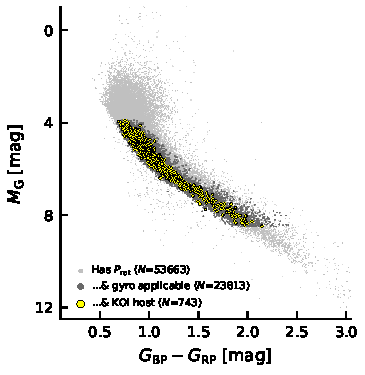
\includegraphics[width=0.48\textwidth]{st_params_M_G_vs_dr3_bp_rp.pdf}
		}
	
		\vspace{-0.3cm}
		\subfloat{
			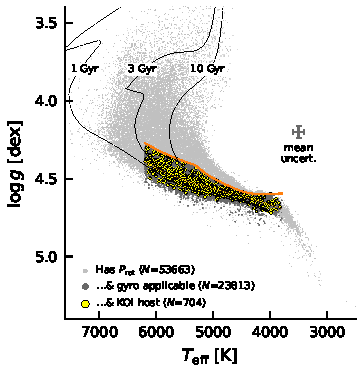
\includegraphics[width=0.48\textwidth]{st_params_adopted_logg_vs_adopted_Teff.pdf}
		}
	\end{center}
	\vspace{-0.5cm}
  \caption{{\bf The stars.}  Our analysis focuses on stars observed by
  Kepler with previously reported rotation periods (gray points).  The
  rotation periods are primarily drawn from
  \citet{Santos_2019,Santos_2021}.  About half of these rotators are
  suitable for gyrochronology (dark gray points), based on factors
  including their non-binarity and proximity to the main
  sequence (see Section~\ref{subsec:flags}).  Some
  host ``confirmed'' or ``candidate'' KOIs that meet additional
  planetary quality criteria (yellow points;
  Section~\ref{subsec:plflags}).  Surface gravities and effective
  temperatures were derived photometrically by
  \citet{Berger_2020a_catalog}.  Isochrones in the lower panel are
  from MIST \citep{Choi_2016}.
	}
	\label{fig:stellarprops}
\end{figure}

This work is focused on Kepler stars for which ages can be inferred
using either rotation, lithium, or both.  Such stars are a minority of
the \nkeplerstars\ Kepler targets.  Rotation periods have been
reported for roughly one in three Kepler targets
\citep[e.g.][]{McQuillan_2014,Santos_2021}.  High-resolution spectra
suitable for measurement of the \ion{Li}{1} 6708\,\AA\ doublet have
only been acquired for the Kepler objects of interest (KOIs), which
comprise a few percent of Kepler's targets.  In the following, we will
describe the set of stars that we adopt with measured rotation periods
(Section~\ref{subsec:rotsel}), the set of objects we adopt as hosting
planets (Section~\ref{subsec:planetsel}), and the subset of these with
high-resolution spectra suitable for lithium analysis
(Section~\ref{subsec:lithiumsel}).  Figure~\ref{fig:stellarprops}
provides a visualization of the various samples.


\subsection{Stellar Rotation Periods}
\label{subsec:rotsel}


\begin{figure*}[!t]
	\begin{center}
		\subfloat{
			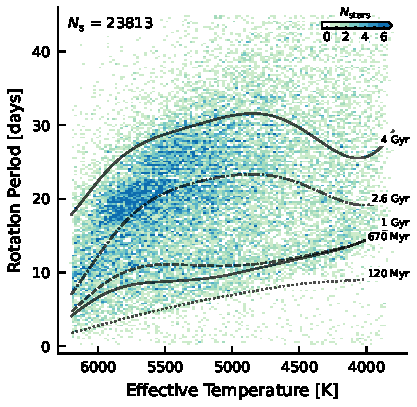
\includegraphics[width=0.49\textwidth]{prot_teff_Santos19_Santos21_dquality.pdf}
		}
		\subfloat{
			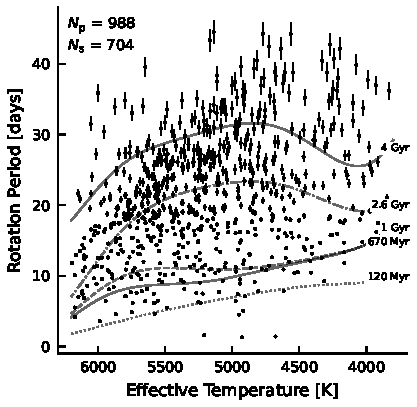
\includegraphics[width=0.49\textwidth]{koi_mean_prot_teff_koi_X_S19S21dquality_keepgrazing.pdf}
		}
	\end{center}
	\vspace{-0.5cm}
	\caption{
    {\bf Rotation periods for Kepler target stars (left) and known
    planet hosts (right)}.  
    The gray lines are ``mean fits'' to the slow rotation sequences of
    open clusters.  The stellar sample (left) includes only apparently
    single stars near the main sequence with $\log g$$>$4.2,
    RUWE$<$1.4, and temperatures of 3800--6200\,K.  The color map has
    a linear stretch.  The planet-hosts (right) require the same
    stellar cuts, and include only the confirmed and candidate planets
    described in Section~\ref{subsec:plflags}.  An order of magnitude
    estimate for the number of young planets discovered by Kepler
    follows by counting planets below the mean rotational isochrones.
	}
	\label{fig:prot_vs_teff}
\end{figure*}


To select stars with rotation periods, we turn to previous work.  Many
investigators have derived rotation periods both specifically for KOIs
\citep{McQuillan_2013,Walkowicz_2013,Mazeh_2015,Angus_2018,David_2021},
and also for the broader set of all Kepler target stars
\citep{McQuillan_2014,Reinhold_2015,Santos_2019,Santos_2021,Reinhold2023}.
These studies used a range of detection methods and selection
functions.  We are interested in understanding the age distribution of
all Kepler target stars irrespective of KOI status.  Out of these
studies, the most homogeneous and precise analyses of both Kepler
targets and KOIs appear to be those by
\citet{Santos_2019,Santos_2021}, hereafter \citetalias{Santos_2019}
and \citetalias{Santos_2021}.  
For a discussion of the work by \citet{Reinhold2023}, please see
Appendix~\ref{app:reinhold23}.
\citetalias{Santos_2019} and
\citetalias{Santos_2021} combined a wavelet analysis and
autocorrelation-based approach, and cumulatively reported rotation
periods for 55{,}232 main-sequence and subgiant FGKM stars.  They
included known KOIs and binaries in their analysis, and removed
transits and eclipses during the stellar rotation measurement process. 

%Studies of stellar rotation across the entire Kepler field include
%those by \citet{McQuillan_2014} (\citetalias{McQuillan_2014}),
%\citet{Reinhold_2015}, \citet{Santos_2019} (\citetalias{Santos_2019}),
%and \citet{Santos_2021} (\citetalias{Santos_2021}).
%\citetalias{McQuillan_2014} used an approach based on the
%autocorrelation function to detect 34{,}030 rotation periods for
%main-sequence Kepler targets cooler than 6500\,K, and excluded known
%eclipsing binaries and KOIs.  \citet{Reinhold_2015} used an iterative
%Lomb-Scargle based approach to analyze $\approx$40{,}000 stars with a
%variability range $R_{\rm var}>0.3$\% that were not known EBs, planet
%candidates, or pulsators; they reported primary rotation periods for
%24{,}124 of these stars.  \citet{Reinhold_2015} also reported
%secondary periods for two thirds of the stars with primary periods,
%which could be caused by differential rotation or finite spot
%lifetimes.  Finally, \citetalias{Santos_2019} and
%\citetalias{Santos_2021} combined a wavelet analysis and
%autocorrelation-based approach, and cumulatively reported rotation
%periods for 55{,}232 main-sequence and subgiant FGKM stars.
%\citetalias{Santos_2019} and \citetalias{Santos_2021} included known
%KOIs and binaries, and assigned them specific quality flags.  The
%rotation periods of KOIs have received considerable additional
%scrutiny
%\citep[e.g.][]{Walkowicz_2013,Mazeh_2015,Angus_2018,David_2021}.

We therefore adopt the results of \citetalias{Santos_2019} and
\citetalias{Santos_2021} as our default rotation periods.
\citetalias{Santos_2021} provided a comparison against
\citetalias{McQuillan_2014}; the brief summary is that the periods
agree for 99.0\% of the 31{,}038 period detections in common between
the two studies.  \citetalias{Santos_2021} classified the 2{,}992
remaining stars from \citetalias{McQuillan_2014} as not showing
rotation periods based on updated knowledge of contaminants
(e.g.~giant stars and eclipsing binaries) and visual inspection.  In
addition, \citetalias{Santos_2021} reported rotation periods for
24{,}182 main-sequence and subgiant FGKM stars that were not reported
as periodic by \citetalias{McQuillan_2014}.  Many of these reported
detections have lower variability amplitudes and longer periods than
those reported by \citetalias{McQuillan_2014}. 

Analyzing the compilation of \citetalias{Santos_2019} and
\citetalias{Santos_2021} rotation periods for the KOI hosts, we
noticed that some known KOIs with rotation periods were missing.  This
is not surprising, since the rotation periods of KOIs have received
considerably more scrutiny than those of ordinary Kepler stars.  We
therefore decided to split our subsequent analysis into a homogeneous
portion that used only the \citetalias{Santos_2019} and
\citetalias{Santos_2021} data, and an inhomogeneous portion that also
considered a broader set of available KOI rotation periods.  For the
latter portion, we first included 32 KOIs with orbital and rotation
periods within $\approx$20\% that had been
excluded %\footnote{Excluding stars in this category would impose a bias
%against young close-in planets, due to the natural commensurability
%between the rotation rates of young stars, and Kepler's increased
%sensitivity to short-period objects.  Although some of these KOIs are
%known false positives, our analysis excludes such objects at later
%steps.}%  As one motivating example, this subset of stars includes {\it
%e.g.}~Kepler~1643 (KIC~8653134), with $P_{\rm orb}$=5.34\,days and
%$P_{\rm rot}$=5.05\,days, which is known to be $\approx$40\,Myr old
%based on membership in RSG-5 \citep{Bouma_2022b}.  }
from the \citetalias{Santos_2019} and \citetalias{Santos_2021}
catalogs (A.~Santos, private communication).  We then incorporated an
additional \nnewdavidtwentyone\ rotation periods for KOI hosts that
\citet{David_2021} had described as either ``reliable'' or ``highly
reliable'' in their visual analysis of previously reported KOI
rotation periods from \citet{McQuillan_2013}, \citet{Walkowicz_2013}, \citet{Mazeh_2015}
and \citet{Angus_2018}.  Inclusion of these additional KOI rotation
periods is a supplementary measure aimed at completeness in our final
KOI age catalog; the provenances of the individual adopted periods are
noted in the relevant tables.

Finally, since our scope is focused on rotation-based ages, we
restricted our attention to stars with reported $P_{\rm
rot}$$<$45\,days.  The slowest-rotating FGK
stars in the open clusters used to
calibrate our gyrochronology model have $P_{\rm rot}$$\approx$35\,days.
Figure~\ref{fig:prot_vs_teff}
shows the resulting \nuniqstarsantosrot\ Kepler stars with rotation
periods compiled from \citetalias{Santos_2019},
\citetalias{Santos_2021}, and our extended KOI list.

To assess the statistical uncertainties of these rotation periods, we
compared our adopted periods with those reported by
\citet{McQuillan_2014}.  The details are in Appendix~\ref{app:reinhold23}.  We found
that for $P_{\rm rot}\lesssim$15\,days, the two datasets agree at a
precision of $\lesssim$0.01$P_{\rm rot}$.  At longer periods of
$P_{\rm rot}\approx$30\,days, the agreement was typically at the
$\lesssim$0.03$P_{\rm rot}$ level, and the envelope of the
period difference increased roughly linearly with period.  Based on
this comparison, we adopted a simple prescription for the period
uncertainties, such that there are 1\% relative uncertainties below
$P_{\rm rot}=15$\,days, and a linear increase thereafter, with slope
set to require 3\% $P_{\rm rot}$ uncertainties at rotation periods of
30 days.







\subsection{Kepler Objects of Interest}
\label{subsec:planetsel}

We considered planets in the NEA cumulative KOI table as of 2023 June
6, which included the best knowledge available on any given planet
candidate while also incorporating human-based vetting.  These planets
represent a superset of those in the fully automated Q1-Q17 DR25 KOI
Table \citep{Thompson_2018}, which could be adopted in future work for
planet occurrence rate calculations.  This version of the cumulative
KOI table included \nkoisnofp\ objects that are either ``confirmed''
or ``candidate'' planets, after excluding known false positives. 

\subsection{High Resolution Spectra}
\label{subsec:lithiumsel}

The final piece of our analysis involves assessing ages based on the
\ion{Li}{1} 6708\,\AA\ doublet.  We analyzed spectra
from the High Resolution Echelle Spectrometer (HIRES;
\citealt{vogt_hires_1994}) on the Keck I 10m telescope.  These spectra
were primarily collected through the California Kepler Survey
\citep{2017AJ....154..107P,2017AJ....154..108J,2017AJ....154..109F}.
We supplemented the existing archive with $\approx$10~hours of new
observations for 22 stars between Fall 2022 and Spring 2024.  These
stars were chosen to ensure that confirmed planets with rotational
evidence for ages below 1\,Gyr had spectra, since this is the age
range in which lithium is most likely to yield useful age constraints.

% stat from _estimate_new_lithium_timefrac.py
Lithium equivalent widths and abundances for the Kepler Objects of
Interest were already analyzed by \citet{2018ApJ...855..115B} for
roughly three quarters of the spectra in our sample.  However, new
spectra have since been acquired, and our approach and selection
function are different.  We therefore performed our own line width
measurements on
the reduced HIRES spectra.

We collected all blaze-corrected HIRES spectra from our group's
observations of non-false positive Kepler Objects of Interest with a
``multiple event statistic'' (MES, {\it koi\_max\_mult\_ev}) of at
least 10.  This yielded at least one spectrum for \nstwithspec\
stars hosting \nplwithspec\ planets.  About half of these stars have
measured rotation periods (\nstwithspecandprot\ stars and
\nplwithspecandprot, respectively).   For stars with multiple spectra
available, we analyzed only
the spectrum with the highest number of counts.  The resulting spectra
were acquired between 2009 September 6 and 2024 May 16, and
cumulatively comprise \nhireshours\,hours of open-shutter time.

We measured the lithium equivalent widths using a procedure adapted
from previous work \citep{Bouma_2021}.  Our stars of interest are FGK
stars, and so the continuum in the vicinity of the \ion{Li}{1}
6708\,\AA\ doublet is well-defined.  We Doppler-corrected the spectra
to a common reference wavelength by cross-correlating against a high
S/N template for Kepler-1698, chosen because $|\gamma|$$<$10\kms,
$T_{\rm eff}$$\approx$5000\,K and $v\sin i$$\approx$5\,\kms, which
puts it in the middle of our sample's temperature range and gives it
mild line-broadening.  We then trimmed the Doppler-corrected spectra
to a local window centered on the lithium line, using a window width
of 15\,\AA\ (we also considered 10\,\AA\ and 20\,\AA; the results were
consistent).  We continuum-normalized by fitting a third-degree
Chebyshev series, while excluding regions with absorption lines.  We
then numerically integrated the resulting spectrum using a
one-component Gaussian with free amplitude, width, and mean, and
estimated uncertainties on the line width through a Monte Carlo
procedure that bootstrapped against the local scatter in the continuum.
The resulting EWs are shown in Figure~\ref{fig:li_vs_teff}.

Our EW measurement approach did not correct for the neighboring
\ion{Fe}{1} 6707.44\,\AA\ blend.  To evaluate the accuracy and
precision of our method, after applying an initial
iteration on the \nlithiumstars\ KOIs with spectra, we compared our
lithium equivalent widths with those reported by
\citet{2018ApJ...855..115B}.  For the \nbergeroverlap\ stars in both
samples, we found broad agreement at $>$30\,m\AA, and significant
differences at $<$30\,m\AA\ because \citet{2018ApJ...855..115B}
required positive EWs, while we allowed for statistically negative ones.  At
$>$30\,m\AA, there is however a small offset in our respective scales caused
by our non-treatment of the iron blend,
such that (B24-B18)$=$7.50$\pm$8.55\,m\AA.
We therefore directly subtracted
this constant mean value (7.50\,m\AA) when calculating lithium-based
ages.  This offset is at worst five times smaller than the astrophysical
scatter present in lithium EWs for calibration clusters at any given age
\citep[see][]{Jeffries_2023}.


\begin{figure}[!t]
	\begin{center}
		\leavevmode
		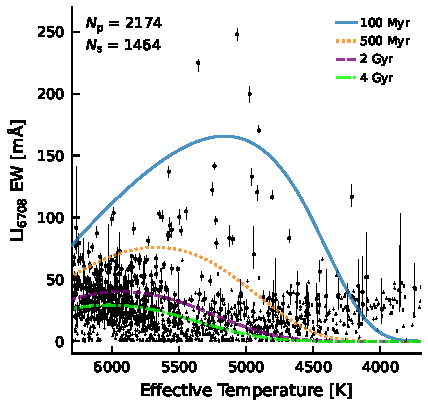
\includegraphics[width=0.49\textwidth]{li_vs_teff_koi_X_JUMP_eagles.pdf}
	\end{center}
	\vspace{-0.25cm}
	\caption{{\bf Equivalent widths (EW) of the \ion{Li}{1} 6708\,\AA\ doublet
    for planet-hosting stars.} These measurements were made from
    Keck/HIRES spectra collected from 2009--2024.  Lines are the ``mean''
    isochrones from \citet{Jeffries_2023}.  The
    intrinsic dispersion around these isochrones becomes much larger
    than changes in the mean at $\gtrsim$1\,Gyr (see
    Figure~\ref{fig:models}).  Some stars with lithium detections do
    not have detected rotation periods, and vice-versa.
		\label{fig:li_vs_teff}
	}
\end{figure}



\section{Stellar Properties}
\label{sec:stellarprops}



% https://gea.esac.esa.int/archive/documentation/GDR3/Data_analysis/chap_cu8par/sec_cu8par_apsis/ssec_cu8par_apsis_gspphot.html

Our default source for stellar temperatures and surface gravities was
the Gaia-Kepler Stellar Properties Catalog (GKSP;
\citealt{Berger_2020a_catalog}).  The GKSP parameters were reported
for stars with ``AAA'' 2MASS photometry, measured parallaxes in Gaia
DR2,  and $g$-band photometry available from either SDSS or else Kepler-INT
\citep{2012AJ....144...24G}.  The parameters themselves were derived using
\texttt{isoclassify} \citep{2017ApJ...844..102H} to interpolate over
the MIST isochrone grids \citep{Choi_2016,2016ApJS..222....8D}, given
the SDSS $g$ and 2MASS $K_{\rm s}$ photometry, the Gaia DR2
parallaxes, and $V$-band extinction from the
\citet{2019ApJ...887...93G} reddening map.  The resulting stellar
parameters are available for \fracstarswithprotwithbtwenty\ of the
\nuniqstarsantosrot\ Kepler stars with rotation periods.  For the
remaining \fracstarswithprotwithoutbtwenty\ of stars that lack
temperatures and surface gravities from
\citetalias{Berger_2020a_catalog}, we adopted the values reported by
\citet{Santos_2019} and \citet{Santos_2021}, which for these cases
primarily derive from the \citet{Mathur_2017} DR25 Kepler Stellar
Properties Catalog, and are mostly derived from photometry.  In the
planet sample, \frackoisnofpwithprotwithbtwenty\ of the
non-false-positive KOIs with rotation periods have parameters from
\citet{Berger_2020a_catalog}, and the remainder are drawn
from DR25. 

\citet{David_2021} compared the photometric
\citetalias{Berger_2020a_catalog} stellar parameters ($T_{\rm eff}$,
$R_\star$, [Fe/H]) against the spectroscopic parameters from
\citet{Fulton_2018}.  The temperature scales showed a few-percent
systematic difference, with \citetalias{Fulton_2018} quoting higher
temperatures than \citetalias{Berger_2020a_catalog} for mid K dwarfs,
and lower temperatures for early F dwarfs.  Our age analysis,
described below, adopts the maximum of the two-sided
uncertainties reported by \citetalias{Berger_2020a_catalog} as a
symmetric Gaussian temperature uncertainty.  Systematic
uncertainties in the temperature scale generally influence 
our age uncertainties at a
smaller level than the statistical intrinsic scatter in the
open cluster rotation sequences.


\begin{figure*}[!t]
	\begin{center}
		\leavevmode
		\subfloat{
			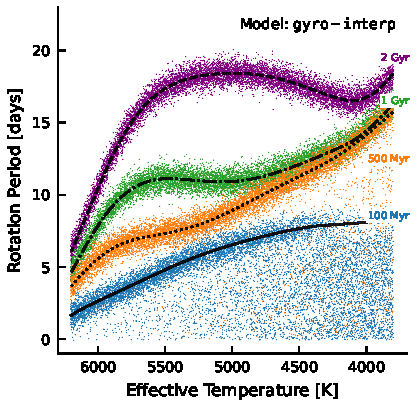
\includegraphics[width=0.49\textwidth]{gyromodeldispersion.pdf}
		}
		\subfloat{
			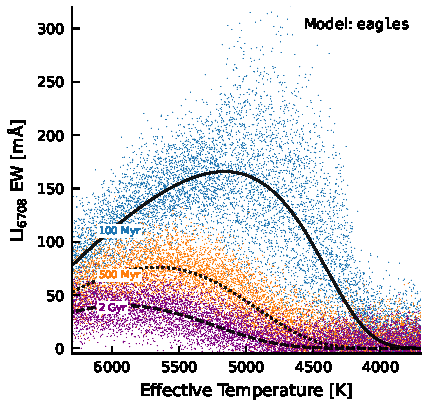
\includegraphics[width=0.49\textwidth]{li_vs_teff_koi_X_S19S21dquality_eagles_showpoints_nodata.pdf}
		}
	\end{center}
	\vspace{-0.6cm}
	\caption{
		{\bf The models.}
		Points represent $10^4$ draws from models that have been fitted to
		rotation periods \citep{Bouma_2023} and lithium equivalent widths
		\citep[EWs;][]{Jeffries_2023} of stars in open clusters.  Lines
		are the ``mean models'' at various ages.  The intrinsic dispersion
		in rotation and lithium about these mean models, which is what the
		models fit, sets the theoretical precision floor for the
		age-dating methods.    Additional sources of uncertainty,
		including measurement uncertainty, impose further limits on
		achievable precision.  These models are calibrated using open
		clusters younger than 4\,Gyr.  The displayed points assume a
		uniform distribution in temperature for visual clarity.  The sizes
		of the points are the same in each panel, so that low apparent
		density signifies greater dispersion around the mean.
		\label{fig:models}
	}
\end{figure*}

\section{Ages From Rotation}
\label{sec:rotage}



We calculated gyrochrone ages using \texttt{gyro-interp}
\citep{Bouma_2023}, which is a method designed to address the fact
that stars with the same mass and same rotation period can have a wide
range of ages \citep[e.g.][]{Curtis_2019_ngc6811}.  The gyrochrone
age posterior should therefore incorporate the intrinsic
population-level scatter into its statistical precision.  Figure~\ref{fig:models} highlights this problem,
particularly in regions where the 0.1--1\,Gyr stars overlap.

To estimate the
stellar spin-down rate as a function of time and stellar temperature,
\texttt{gyro-interp} uses measured rotation periods and effective
temperatures from reference open clusters, and interpolates between them using cubic
Hermite polynomials.  We calculated the probability of the
rotation-based age, $t_{\rm gyro}$, given the observed 
periods and temperatures (and their uncertainties) by
integrating Equation~1 of \citet{Bouma_2023}.  This procedure marginalizes over the 
astrophysical scatter that is observed in the open cluster
sequences.
We adopted a linear age grid spanning 0--5\,Gyr with
500 grid points, and interpolated the resulting posteriors to calculate
any summary statistics.
The oldest cluster for which
\texttt{gyro-interp} is calibrated 
is the 4\,Gyr M67 cluster
\citep[][]{Dungee_2022,Gruner_2023}.  
For Kepler stars with rotation periods above the 
M67 sequence, our resulting age constraints are quoted as lower limits.



\subsection{Stellar Quality Flags}
\label{subsec:flags}
We calculated gyrochrone ages for all \nuniqstarsantosrotteffcut\
stars with reported rotation periods that had effective temperatures of
3800--6200\,K.  To identify stars for which we suspect these ages may not
be valid, we built a set of quality flags which we then condensed
into a single binary number: $Q_{\rm star}$.  When and how
this bitmask should be applied depends on the question being
asked.  If the goal is to construct a false-positive free sample, all the
quality flags could be applied.  If the goal is to construct a complete sample,
then consider the examples of Kepler~1627Ab ($\approx$40\,Myr) and
Kepler~51c ($\approx$625\,Myr).  The former has a high RUWE due to a
resolved binary companion \citep{Bouma_2022a}; the latter is on a
grazing orbit \citep{2014ApJ...783...53M}.  We leave selection for or
against such cases as a decision to the user.
For our own analysis, 
we assume that a star
is suitable for gyrochronology if none of bits zero through nine
(inclusive) are raised.  For analyses that require all
stellar rotation periods to come from the same detection pipeline, we
further require bit 11 to be zero. 

Three assumptions must hold for a rotation-based age dating method
like \texttt{gyro-interp} to be valid.  {\it 1)} The evolutionary
state of the star must be well-specified by its temperature and its
age, {\it 2)} the star's spindown must not be influenced by binary
companions, and {\it 3)} the rotation period distribution for field
stars of a given temperature and age must be identical to that of
equally aged open clusters (metallicity differences, for instance, are
ignored).  A rephrasing of the first condition is that the star must
be ``near the main sequence'' because during the post main sequence
stellar temperatures change.  From $\approx$0.08 to $\approx$3\,Gyr,
the stars of interest in this work (3800--6200\,K,
0.5--1.2\,$M_\odot$) have temperatures constant to $\approx$1\%
\citep{Choi_2016}.  From $\approx$3--4\,Gyr, a 1.2\,$M_\odot$ star's
temperature drops from $\approx$6200\,K to $\approx$6000\,K
($\approx$3\%), because its outer layers expand as it begins hydrogen
shell burning as a subgiant.  We treat this issue in a manner
discussed in ``bit 9'' below.

{\it Temperature range (bit 0)}---We require stars to have effective
temperatures $T_{\rm eff}$ between 3800 and 6200\,K in order to report
gyrochrone ages \citep{Bouma_2023}.   Stars hotter than 6200\,K spin
down very slowly, if at all.  Stars cooler than 3800\,K do spin down
over gigayear timescales
\citep{2016ApJ...821...93N,2023ApJ...954L..50E,2024arXiv240312129C},
but the currently available open cluster data have yet to clarify
when the intrinsic scatter in the population decreases.

{\it Surface gravity (bit 1)}---We flagged stars as possible subgiants
if they had $\log g < 4.2$.  We set this threshold by examining the
relevant flag from \citet{berger_2018_radii_evolnstates},
cross-matched against \citet{Berger_2020a_catalog}.

{\it Absolute luminosity (bit 2)}---We calculated the absolute Gaia
DR3 $G$-band luminosity, ignoring reddening, using the reported
apparent $G$-band magnitude and parallaxes.  We flag stars with
$M_{\rm G} < 3.9$ or $M_{\rm G} > 8.5$, corresponding to main-sequence
spectral types earlier than $\approx$F8V or later than $\approx$M0.5V
\citep{Pecaut_2013}.

{\it Known eclipsing binaries (bit 3)}---We flagged any stars reported
to be in the final Kepler eclipsing binary catalog (KEBC;
\citealt{2016AJ....151...68K}).

{\it Kepler-Gaia crossmatch quality (bits 4 and 5)}--- In situations
where we wanted to leverage Gaia DR3 data, we used M.~Bedell's 4$''$
Kepler-to-Gaia crossmatch %\footnote{\url{https://gaia-kepler.fun}, last
%accessed 15 April 2024.  We used 4$''$ rather than the 1$''$ match
%because 91 KOIs are omitted in the 1$''$ match, 23 of which have
%either ``candidate'' or ``confirmed'' status.  Almost all of these 23
%are M dwarfs with high proper motions.  Performing the same crossmatch
%at 4$''$, only two KOIs (KOI-3993 and KOI-6531), both known
%false positives, fail to yield Gaia DR3 crossmatches.}, 
%which is a
%crossmatch
of the NEA \texttt{q1\_q17\_dr25\_stellar} catalog with Gaia DR3
(available at \url{https://gaia-kepler.fun}).  The
separation distribution of the Kepler-Gaia DR3 crossmatches is such
that 99.2\% of candidate matches are within 1$''$.   We nonetheless
noted an upturn in the candidate match rate from 3-4$''$; such sources
are flagged using bit 4.  For KIC stars with multiple potential Gaia
matches within the 4$''$ radius, we adopted the brightest star as the
default match.  In most such cases this was unambiguous because there
is a large brightness difference between the primary and any apparent
neighbors.  However cases with multiple stars within 4$''$ within
$\Delta G$$<$$0.5$\,mag are noted using bit flag 5.  

{\it Gaia DR3 non-single-stars (bit 6)}---The Gaia DR3
\texttt{non\_single\_star} column in the \texttt{gaia\_source} table
flags known eclipsing, astrometric, and spectroscopic binaries.  We
directly included this column.

{\it RUWE (bit 7)}---We inspected diagrams of the Gaia DR3
renormalized unit weight error (RUWE) as a function of other stellar
parameters, and flag stars with RUWE$>$1.4 as possible binaries.  Such
astrometric outliers can be either bona fide astrometric binaries, or
more often are marginally resolved point sources for which a
single-source PSF model provides a poor fit.

{\it Crowding (bit 8)}---We searched the Gaia DR3 point source catalog
for stars within 1 Kepler pixel (4$''$) of every target star.  While
such companions may not not be physically associated with the target
star, their presence can confuse rotation period measurements.  We
therefore flagged any stars with neighbors down to 10$\times$ the
brightness of the target star within this region ($\Delta G < 2.5$).

{\it Near the main sequence (bit 9)}---Figure~\ref{fig:stellarprops} shows
that many stars observed by Kepler
are far from the main sequence.  Some of the challenges this introduces
for rotation-based ages include unresolved binaries, metallicity,
reddening, and drivers of rotation other than magnetic braking.
After exploring various options, we settled on the orange locus in the
$\log g$--$T_{\rm eff}$ plane shown in Figure~\ref{fig:stellarprops}
as a way of flagging unresolved binaries, as well as evolved
late-F and early-G stars.  While the exact details of how this locus
is constructed are arbitrary (see Appendix~\ref{app:linemethod}), the
general aim is to flag stars for which there is evidence based on
their location in the HR diagram that our gyrochronology model may not
be reliable.  While the $\log g$--$T_{\rm eff}$ cut flags about half
of Kepler stars with rotation periods as potentially not being
suitable for gyrochronology, a few outliers in $M_{\rm G}$ vs.~$G_{\rm
BP}$-$G_{\rm RP}$ remained after applying it.  Such outliers are
likely also questionable.  We therefore also fitted a polynomial to
the KOI main sequence in $M_{\rm G}$ vs.~$G_{\rm
	BP}$-$G_{\rm RP}$, and flagged stars more than 1\,magnitude from
this locus as part of the same bitflag.

%The rotation period
%distribution of sources excluded in this manner includes a relatively
%larger fraction of ``rapid rotators'' than the main sequence sources,
%likely due to a combination of astrophysical and systematic effects.
%See for instance Figure~8a of \citet{2022AJ....164..137K} or
%Figures~12 and 13 of \citet{2023ApJS..268....4F} for examples of how
%the period distribution of this population differs from stars near the
%main sequence.


{\it Candidate pulsators and close-in binaries (bit
10)}---\citeauthor{Santos_2021} included in a flag for candidate
``classical pulsators'' (e.g.\ Cepheids) and close-in binaries.
Visual inspection shows that although this flag selects many bona fide
objects in these classes, it also selects most $P_{\rm
rot}$$\lesssim$5\,day bona fide young planets.  These objects are
neither classical pulsators nor close binaries.  While we propagated
this flag into our set of quality flags, we therefore generally ignore
it.

{\it Not in the homogeneous stellar rotation sample (bit 11)}--- This
flag is set for the KOIs with rotation periods drawn from a source
other than the \citeauthor{Santos_2019} pipeline.




\subsection{Planet Quality Flags}
\label{subsec:plflags}
Some planets are more reliably identified than others.  We use the
following additional quality indicators to assess the reliability and
utility of a planet, and assemble them into a separate bitmask,
$Q_{\rm planet}$.

% see Erik's 2022 discussion; might want to shift to include a cut on
% disposition score?
{\it Candidate reliability (bit 0)}---The NEA's Kepler Objects of
Interest Table includes both an overall planet-candidate disposition
status ({\it koi\_disposition}), as well as a disposition based only
on the Kepler data ({\it koi\_pdisposition}).  We require both to
include only ``planet candidates'' and ``confirmed planets''. 
%; we are generally less interested
%in the age distribution of planet candidates that are known false positives.

{\it Candidate S/N (bit 1)}---In any transit survey, the false
positive rate increases greatly toward the noise floor for planet
detection \citep[e.g.][]{2002ApJ...564..495J}.  We required a S/N in
excess of Kepler's usual 7.1$\sigma$ floor, through a cut on the
maximum ``multiple event statistic'' (MES, {\it koi\_max\_mult\_ev}):
we required ${\rm MES}$$>$10.

{\it Grazing planets (bit 2)}---Grazing objects, for which the impact
parameter $b$ is greater than $1-R_{\rm p}/R_\star$, often yield
biased planetary parameters \citep[e.g.][]{2022AJ....163..111G}.  For
large planets, they also include astrophysical false positives at
higher rates \citep{2016ApJ...822...86M}, in part due to the
size-impact parameter degeneracy.  We flag planet candidates as
potentially grazing if $b$$>$0.8, using the impact parameters reported
by \citet{Thompson_2018}.




\section{Ages From Lithium}
\label{sec:liage} 

Figure~\ref{fig:li_vs_teff} shows our measured equivalent widths for
the lithium 6708\,\AA\ absorption doublet, plotted over the mean
isochrone models from \texttt{EAGLES} \citep{Jeffries_2023}.  We
show an upper-limit for plotting purposes if the 1$\sigma$ lower
limit on the equivalent width is below 10\,m\AA.  Our measured EWs
span -40 to 250\,m\AA; all negative EWs have uncertainties that are
statistically consistent with zero.

To calculate lithium ages, we use \texttt{EAGLES} (git commit
\texttt{ac09637}), which, similar to \texttt{gyro-interp}, is based on
an empirical interpolation approach.  \texttt{EAGLES} 
was calibrated on lithium measurements of stars observed by the
Gaia-ESO spectroscopic survey in 52 open clusters with ages spanning 2
to 6{,}000\,Myr \citep{Jeffries_2023}.  We adopt a linear prior in
age, spanning $10^6$ to $10^{10}$\,yr, and symmetrize our EW
uncertainties for purposes of interfacing with \texttt{EAGLES} by
taking the maximum of the measured positive and negative 1$\sigma$
uncertainty intervals.

In part because many of our EWs are upper limits, many of the lithium
ages are lower limits.  In such cases,  the inferred age posterior is
strongly influenced by the assumed intrinsic dispersion in
the lithium model, and by the prior.  In these instances, we
quote the 3$\sigma$ (99.7$^{\rm th}$ percentile) limits.


%\subsection{Sample Summary}
%\label{subsec:tally}
%
%The rotation periods for the star and planet samples are shown in
%Figure~\ref{fig:prot_vs_teff}.  Out of the \nkeplerstars\ stars
%observed by Kepler, requiring reported rotation periods and a reliable
%DR3 crossmatch yields \nuniqstarsantosrot\ stars.  Further requiring
%these stars to have temperatures of 3800--6200\,K yields
%\nuniqstarsantosrotteffcut\ stars.  Further requiring the stars to be
%apparently single, near the main sequence, with $\log g$$>$4.2,
%$M_{\rm G}>3.9$, and not flagged as eclipsing binaries yielded
%\nuniqstarsantosallbutruwe\ rotators.
%Finally, imposing the full set of quality cuts,
%i.e.~further requiring RUWE$<$1.4 and requiring no
%resolved blends ($\Delta G$<2.5) within 4$''$ leaves
%\nuniqstarsantosrotgyroappl\ stars for which we expect rotation-based
%age dating to be secure.
%
%
%In the planet sample, the cumulative KOI table included
%\nnonfpcumkois\ confirmed and candidate planets, orbiting
%\nnonfpcumkoihosts\ stars.  Assume that we apply all the same stellar
%cuts, save for that on RUWE.  We can then require these confirmed and
%candidate planets to have MES$>$10.  This combination of selection
%criteria yield \nplwgyroagewithgrazingandhighruwe\ planets with
%rotation-based ages orbiting
%\nplhoststarwgyroagewithgrazingandhighruwe\ stars
%(\nplhoststarwgyroagejusthighruwe\ of these stars with ``high'' RUWE).
%If we additionally require the planets to be non-grazing ($b<0.8$), we
%are left with \nplwgyroagenograzing\ planets orbiting
%\nplhoststarwgyroagenograzing\ stars with rotatio-based ages.
%This cut drops $\approx$41 more planets than one would expect if the initial sample
%of \nplwgyroagewithgrazingandhighruwe\ planets had zero false positives.
%The binomial probability that this could happen by coincidence is 0.1\%.




\section{Cluster Age Comparison}
\label{sec:litagecomparison}



\begin{figure*}[!t]
	\begin{center}
		\subfloat{
			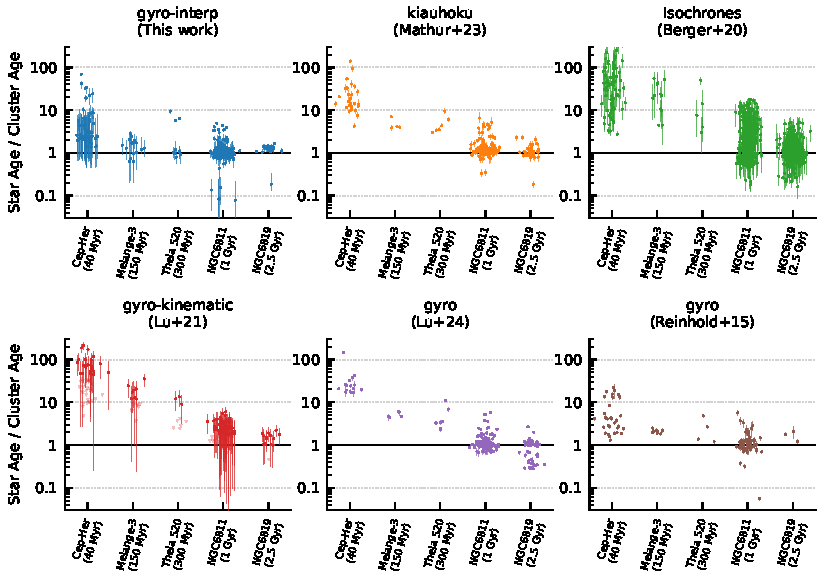
\includegraphics[width=0.96\textwidth]{olympic_merged_lit_ages_vs_cluster_ages.pdf}
		}
	\end{center}
	\vspace{-0.5cm}
	\caption{
		{\bf Reported ages of individual stars in benchmark open clusters.}
		Each point denotes a reported age,
		normalized by the age of a stellar ensemble in which the star
		is a candidate member.
		Cluster membership was assessed in previous studies without knowledge of rotation.
		Although some field interlopers may be present in the 
		membership lists,
		outliers can be compared between different methods on a
		relative basis.
    Each study was cross-matched against the same cluster list;
    certain methods report ages for more stars than others.
		Horizontal scatter is artificially added to visually
		clarify the statistical age uncertainties.
	}
	\label{fig:agescalecompone}
\end{figure*}

Stars that formed in the same birth cluster are the gold standard for
the astronomical age scale \citep{Soderblom_2010}.  Before Gaia, the
few open clusters known in the Kepler field had been
cataloged by \citet{1864RSPT..154....1H}.  Gaia
has enabled the discovery of stellar ensembles
that are more diffuse, but which nonetheless share a common age based
on e.g.~isochrone, rotation, and lithium dating
\cite[e.g.][]{2019AJ....158..122K,Bouma_2022b,Barber_2022}.

In Figure~\ref{fig:agescalecompone}, we compare our rotation-based
ages, and available ages from the literature, against the ages of
stars in open clusters in the Kepler field.  From the
literature, we drew ages from \citet{Reinhold_2015},
\citet{Berger_2020a_catalog}, \citet{2021AJ....161..189L},
\citet{2023ApJ...952..131M}, and \citet{2024AJ....167..159L}.  We
followed any guidance available from each study for
removing ages that were flagged as unreliable, and plotted
stars within $1\sigma$ of zero upper limits.  For the
\citeauthor{Reinhold_2015} ages, we used those calculated
using the \citet{Mamajek_2008} calibration; for the
\citeauthor{2023ApJ...952..131M} ages, we show those from
\texttt{kiauhoku} \citep{Claytor2020} rather than \texttt{STAREVOL}
\citep{Amard2019}, since the former showed better agreement with
the cluster age scale.

Cluster membership is a nuanced subject.
Figure~\ref{fig:agescalecompone} is showing reported ages for a set of
spatially and kinematically selected stars that could be
cluster members, or they could be field interlopers.  For NGC6811 and
NGC6819, we adopted candidate members from
\citet{2018A&A...618A..93C,CantatGaudin_2020} and
\citet{Kounkel_2020}.  
For Theia~520, we used candidate members from \citet{Kounkel_2020}.
For Melange-3 we used the candidates reported
by \citet{Barber_2022} and required ``offset'' tangential velocities
below 2\,\kms.  For Cep-Her we used candidate members from Kerr et al.~2024 (submitted)
with $P_{\rm fin}$$>$0.8.  Even with
contaminants, we can compare the relative age distributions derived by
the different studies because in all instances we are comparing
reported ages against a fixed list of stars.

There are two main metrics for success in this test. {\it 1)}
Do the reported ages agree with the cluster age? {\it 2)} Do the
reported age uncertainties agree with their dispersion
around the cluster age?

Figure~\ref{fig:agescalecompone} show that although
previous studies reported ages that agree with the cluster scale for
$\gtrsim$1\,Gyr stars, sub-gigayear stars have historically had their ages 
overestimated by 0.3--2\,dex, with severely understated uncertainties.  
For isochrone and kinematic ages, this is because these
methods rely on parameters that do not appreciably change at
$t$$\lesssim$1\,Gyr.  For the rotation-based ages in
\citet{2023ApJ...952..131M} and \citet{2024AJ....167..159L}, the
discrepancy is
caused by details of the calibration methodologies.  The
\texttt{kiauhoku} spin-down model for instance has known
``stretches'' and ``compressions'' in its age scale relative to observed open clusters
\citep[see][Sec. 7.3]{2023ApJ...952..131M}.
The \citet{Mamajek_2008}
calibration used by \citet{Reinhold_2015} appears more accurate than the former
two models, because it 
was fitted to reproduce the open cluster sequences known at the time.  However the
uncertainties from all of these methods appear to be underestimated.  This
is probably because
they do not marginalize over
the range of rotation periods accessible to stars of a fixed
mass and age.



\section{Results}
\label{sec:results}

\begin{figure*}[!t]
  \begin{center}
    \leavevmode
    \subfloat{
%    \includegraphics[width=.96\textwidth]{comp_hist_samples_koi_gyro_ages_hist_field_gyro_ages_20240430_maxage4000.pdf}
%    \includegraphics[width=.96\textwidth]{comp_hist_samples_koi_gyro_ages_hist_field_gyro_ages_20240521_maxage4000.pdf}
        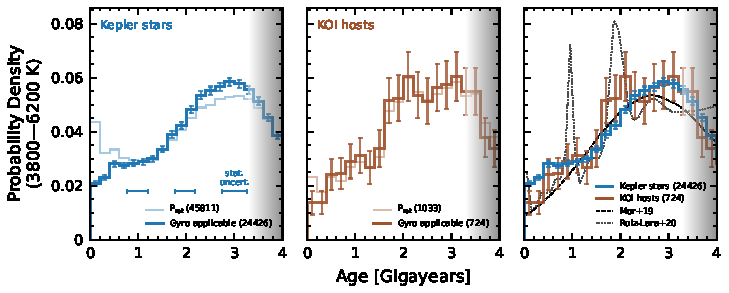
\includegraphics[width=.96\textwidth]{comp_hist_samples_koi_gyro_ages_hist_field_gyro_ages_20240530_maxage4000.pdf}
    }

	\vspace{-0.35cm}
    \subfloat{
%    \includegraphics[width=.96\textwidth]{comp_hist_samples_koi_gyro_ages_hist_field_gyro_ages_20240430_maxage4000_preciseagesonly.pdf}
%    \includegraphics[width=.96\textwidth]{comp_hist_samples_koi_gyro_ages_hist_field_gyro_ages_20240521_maxage4000_preciseagesonly.pdf}
        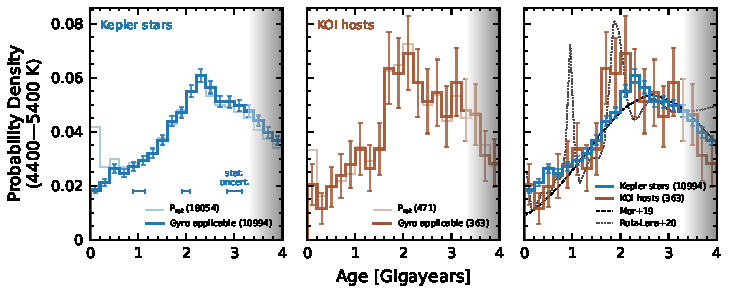
\includegraphics[width=.96\textwidth]{comp_hist_samples_koi_gyro_ages_hist_field_gyro_ages_20240530_maxage4000_preciseagesonly.pdf}
    }
  \end{center}
  \vspace{-0.66cm}
  \caption{{\bf Kepler's demographic cliff,} visible in the
  rotation-derived ages of stars (left) and planet hosts (middle) in
  the Kepler field.  The top row shows all stars with
  temperatures of 3800--6200\,K for which we calculated rotation-based
  ages.  Opaque lines impose quality cuts on 
  binarity, crowding, and the star's evolutionary state; transparent lines do not.
  The bottom
  shows stars with temperatures of 4400--5400\,K, which have
  more precise ages due to their fast spin-down.
  The statistical uncertainty for a mean
  individual star at 1, 2, and 3\,Gyr is shown, and is identical
  across each row.  Finally, the right panel compares the
  rotation-derived ages against star formation histories
  derived using CMD fitting (dashed and dotted lines).  Completeness in Kepler's
  $P$$_{\rm rot}$ detection sensitivity is near unity until
  $t$$\lesssim$3\,Gyr \citep{2022ApJ...937...94M}.
  \label{fig:hist_tgyro}
  }
\end{figure*}


\subsection{A Paucity Of Young Stars And Planets}

The stellar ages are given in Table~\ref{tab:planets} for the known
planet hosts, and in Table~\ref{tab:stars} for all Kepler stars.
Figure~\ref{fig:hist_tgyro} shows the rotation-based age distributions
of all the stars (left column) and the KOI hosts (middle column).
These ``histograms'' are sampled from the posterior probability
distributions by drawing ten random samples from each posterior, and
then computing the re-weighted histogram of the resulting samples.
The uncertainties assume Poisson statistics.  We truncated the plots
near $4$\,Gyr since this is the cluster age out to which our
interpolation-based method is well-calibrated.  The overall slope
yields a paucity of young stars relative to the expectation of a
uniform age distribution.
%In an alternative coinage, this tendency for fewer young
%stars to be present could also be dubbed a ``demographic cliff'',
%in reference to the phenomenon from human demography.

The age distributions of Kepler stars and KOI hosts in
Figure~\ref{fig:hist_tgyro} appear similar.  One diagnostic for
whether the two distributions are drawn from the same underlying
distribution is the Kolmogorov-Smirnov test;  we calculated this
statistic in a manner that accounts for the Poisson uncertainties by
performing 1000 random draws of 70\% of the stars from each sample
when requiring $t_{\rm gyro}$$<$3\,Gyr.  The resulting $\log_{\rm
10}p$ values spanned (2.5$^{\rm th}$ to 97.5$^{\rm th}$ percentiles)
-4.5 to -1.8 for the K dwarfs, and -4.5 to -1.9 for all Kepler stars.
This agrees with the visual impression that while small differences
may be present, they are not drastic.

The similarity of the KOI host and Kepler star age distributions adds
some nuance to the argument that young transiting planets are hard to
detect due to the photometric variability of their host stars.  If
true, this statement seems to hold only for the very youngest
($\lesssim$0.4\,Gyr) stars, where there is a marginal deficit in the
KOI host age distribution relative to that of the overall stellar
sample.  Examining scatter plots of the planet properties as a
function of time, we similarly find that fewer systems at $t_{\rm
gyro}$$<$0.4\,Gyr are detected with $P_{\rm orb}$$\gtrsim$30\,days
than at $t_{\rm gyro}$$>$0.4\,Gyr.

An important separate selection effect concerns Kepler's ability to
detect the rotation signals.  \citet{2022ApJ...937...94M} studied this
issue, and found for Sun-like stars that the fraction of rotation
signals detectable by Kepler is near unity up to $\approx$3\,Gyr, and
that it drops to almost zero by $\approx$5\,Gyr.  This trend is
opposite in functional form to our derived age distributions.

We can quantify the relative counts of stars as a function of age by
labelling stars between 0-1\,Gyr, 1-2\,Gyr, and 2-3\,Gyr as ``young'',
``intermediate-age'', and ``old''.  A simple counting exercise from
Figure~\ref{fig:hist_tgyro} tells us that there are \ratioobtoybstars\
times as many old stars in the Kepler field as young stars.
Similarly, there are \ratioobtoybplanets\ times as many old planet
hosts as young planet hosts.  Focusing only on the tails of the
distributions (0-0.3\,Gyr and 2.7-3\,Gyr), the implication is that the
formation rate of stars in the Kepler field decreased by a factor of
\ratiosfr$\pm$\uncratiosfr\ over the past three billion years.  If
this decrease continues linearly into the future, then a simple
extrapolation would imply that in $\approx$1.4$\pm$0.3\,Gyr the rate
of new stars forming in the Galaxy will reach zero.

In terms of detected planet counts, our rotation-based ages for the
Kepler sample yield \{\nplyounggyro, \nplmidgyro, \nploldgyro\}
detected planets in the 0-1\,Gyr, 1-2\,Gyr, and 2-3\,Gyr bins.  


\subsection{Planets Younger Than One Billion Years}

Sub-gigayear planets can be particularly informative for studies of planet
evolution.
Our catalog has \nplyounggyro\ confirmed planets
with median ages below 1\,Gyr.  Requiring $t_{\rm gyro}$$<$1\,Gyr at
2$\sigma$ yields \nplyounggyrotwosigma\ planets orbiting
\nplhostsyounggyrotwosigma\ stars.  
The youth claim is most secure for the subsets that are either
in clusters, or that have independent rotation and
lithium-based ages.

\subsubsection{Planets in Clusters}
\label{subsec:clusterplanets}

Four stellar ensembles in the Kepler field have to date yielded a
total of fourteen transiting planets.  Our analysis blindly recovers
the youth of all of these planets.

{\it Cep-Her}---The Cep-Her complex ($\approx$40\,Myr)
contains Kepler-1627Ab, Kepler-1643b,
Kepler-1974b and Kepler-1975\,Ab \citep{Bouma_2022b,Bouma_2022a}.
Different sub-groups of the complex vary in age by $\approx$50\%
(Kerr~et al.,~submitted).  The planets
themselves are all on close-in orbits (5-25\,days), with sizes from
2-4\,$R_\oplus$.  Our rotation and lithium ages agree with the cluster age
for Kepler-1627A, Kepler-1974, and Kepler-1975A.  For Kepler-1643, the
rotation and cluster ages agree, and the lithium age is 2.0$\sigma$
above the cluster age reported in \citet{Bouma_2022b} for RSG-5.

{\it MELANGE-3}---\citet{Barber_2022} reported a
$105\pm10$\,Myr association in the Kepler field
containing two transiting mini-Neptunes:
Kepler-970 and Kepler-1928.  We find rotation-based ages
of $t_{\rm
gyro}=176_{-40}^{+120}$\,Myr and $144_{-88}^{+104}$\,Myr for
Kepler-970 and Kepler-1928 respectively.  The former rotation-based
age being slightly older than the suggested Pleiades age for the
association agrees with Figure~4 of \citet{Barber_2022}.

{\it Theia~520}---We derive rotation-based ages of $\approx$350\,Myr
for Kepler-968 and Kepler-52.  Based on spatial and kinematic
clustering, these stars were reported by \citet{2019AJ....158..122K}
to be members of Theia~520.  The core of this
structure is also known as UBC-1 \citep{2018A&A...618A..59C}.  Based
on isochrone and rotation-based age-dating, Theia~520 seems to be
$\approx$230$\pm$70\,Myr old
\citep{2019AJ....158..122K,2024A&A...681A..13F}, which is within 
1$\sigma$ of our $t_{\rm gyro}$
measurements.  Ongoing work by \citet{Curtis2024} broadly finds that
the two planet-hosting stars are indeed members of this diffuse
population.  Given the cluster-level and individual-star evidence,
this makes Kepler-968 and Kepler-52 the youngest multiplanet systems
currently known from the main Kepler mission.

{\it NGC~6811}---\citet{Meibom_2013} reported the discovery of
Kepler-66 and -67b, two mini-Neptunes in NGC~6811 ($\approx$1\,Gyr).
We derive rotation-based ages for these systems of
\kepsixsixtgyro\,Myr and \kepsixseventgyro\,Myr for Kepler-66 and
-67b, respectively.  Kepler-66 ($T_{\rm eff}$$\approx$5900\,K, $P_{\rm
rot}$$\approx$10.4\,days) has a lower precision and a more asymmetric
posterior because of its slow spindown rate.  Kepler-67 ($T_{\rm
eff}$$\approx$5100\,K, $P_{\rm rot}$$\approx$10.3\,days) is marginally
hotter than the later K dwarfs that are in ``stalled'' spindown at
this time, enabling its rotation period to be diagnostic of its age.

\begin{figure}[!t]
  \begin{center}
    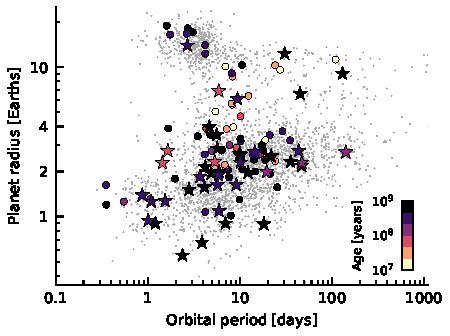
\includegraphics[width=0.48\textwidth]{rp_vs_period_scatter_20240415_colorbyage_showaux-gyro_anyyoung_anyyoung.pdf}
  \end{center}
  \vspace{-0.5cm}
  \caption{
    {\bf Sizes, orbital periods, and rotation-based ages of transiting
    exoplanets younger than one billion years.} Stars denote
    \nplyounggyrotwosigmanograzingnoruwe\ planets that are 
    characterized in this work to have $t_{\rm gyro}$<1\,Gyr at
    $2$$\sigma$; circles are planets from the literature meeting the
    same age requirement, but with a heterogeneous set of age
    provenances.  Gray points are transiting planets from the NASA
    Exoplanet Archive older than 1\,Gyr.  If one were to instead
    select for precise ages ($t/\sigma_{\rm t}>3$), this would hide
    $\approx$ten $<$0.5\,Gyr planets, and add $\approx$fifteen
    0.5-1\,Gyr planets.  For this plot, we require our Kepler stellar
		hosts to not have $Q_{\rm star}$ bits 0--9 raised, and for the planets 
		to similarly no have quality flags raised. 
    \label{fig:rp_period_age_results}
  }
\end{figure}

\subsubsection{Rotation vs.~Lithium Ages}

We compared 
the rotation and lithium ages for the
known planet hosts 
in the ``comment'' column of Table~\ref{tab:planets}.
There were three cases of interest.
{\it i)} If two-sided posteriors for both $t_{\rm gyro}$ and $t_{\rm Li}$ existed,
and their median values were consistent within 2$\sigma$, we listed them
as consistent; if they were consistent within 2-3$\sigma$, we
listed them as ``maybe'' consistent.  Otherwise, they
disagreed.
{\it ii)}
If $t_{\rm Li}$ was a lower limit, we compared this lower limit
with the $1\sigma$ upper limit from $t_{\rm gyro}$; if the two
overlapped, we judged the age estimates to be consistent.
{\it iii)}
If $t_{\rm Li}$ provided a two-sided posterior, and no
rotation period was found, we judged the age estimates to be
inconsistent.  This is because a two-sided lithium constraint can only be
provided for G and K dwarfs $\lesssim$2\,Gyr old, and Kepler should
have been sensitive to the rotation periods of such stars.


%\begin{enumerate}[leftmargin=*,topsep=0pt,itemsep=-1ex,partopsep=1ex,parsep=1ex]
%  \item Two-sided posteriors for both $t_{\rm gyro}$ and $t_{\rm Li}$:
%    if their values were consistent within 2$\sigma$, we judged them
%    to be consistent; if they were consistent within 2-3$\sigma$, we
%    suggest them to be ``maybe'' consistent.  Otherwise, they
%    disagree.
%    %
%  \item If $t_{\rm Li}$ is a lower limit, we compare this lower limit
%    with the $1\sigma$ upper limit from $t_{\rm gyro}$; if the two
%    overlapped, we judge the age estimates to be consistent.
%    %
%  \item If $t_{\rm Li}$ provides a two-sided posterior, and no
%    rotation is reported, we judge the age estimates to be
%    inconsistent.  This is because this lithium constraint can only be
%    provided for G and K stars $\lesssim$2\,Gyr old, and Kepler should
%    have been sensitive to the rotation periods of such stars.
%\end{enumerate}

In the entire planet sample (i.e.~without imposing any quality cuts) this
yielded \allagesyesconsistent\ consistent cases,
\allagesmaybeconsistent\ maybe consistent cases, and
\allagesnoconsistent\ inconsistent cases.  Rephrased, in the overall
sample, \fracconsistentallages\% of stars have consistent rotation and
lithium-based ages (\fracpotentiallyconsistentallages\% potentially
consistent).

Appendix~\ref{app:inconsistent} describes all cases of ``discrepant''
confirmed planets for which a sub-gigayear age is reported by at least
one age indicator.  All but two systems are either evolved stars or
else unresolved binaries, and are automatically flagged as such.  The
more interesting of the two is Kepler-786, an early K dwarf with
$t_{\rm Li}$=\kepseveneightsix\,Myr, but with a $\approx$33\,day
rotaton period that would imply $t_{\rm
gyro}$=\kepseveneightsixgyro\,Myr.  Other age indicators in the
spectrum similarly suggest that the star is not young. 



\subsubsection{New Young Planets}

Let us focus on blemish-free stars with blemish-free planets: $Q_{\rm
star}$ must not have any of bits zero through nine raised, and $Q_{\rm
planet}$ must similarly have no quality flags raised.  Under this
constraint, our results include \ltonegyrhighqconfirmedtwosided\
confirmed planets younger than 1\,Gyr with two-sided $t_{\rm gyro}$
and $t_{\rm Li}$, and \ltonegyrhighqconfirmedonesided\ confirmed
planets with comparable ages for which $t_{\rm gyro}$ is two-sided
while $t_{\rm Li}$ is one-sided.

Figure~\ref{fig:rp_period_age_results} shows the planets and planet
candidates with $t_{\rm gyro}$$<$1\,Gyr at 2$\sigma$.  This figure
includes \nconfirmedplyounggyrotwosigmanograzingnoruwe\ confirmed
Kepler planets, and \ncandidateplyounggyrotwosigmanograzingnoruwe\
candidate planets, all of which are listed in Table~\ref{tab:planets}.
These include \nearthshighq\ objects Earth-sized or smaller,
\njupitershighq\ Jovian-sized planet candidates, \nsubsaturnshighq\
super-Neptunes (4--10\,$R_\oplus$), \nminineptuneshighq\ mini-Neptunes
above the radius valley as parametrized by
\citealt{2018MNRAS.479.4786V}, and \nsuperearthshighq\ super-Earth
sized planets below the radius valley.  While most of these planets
are on orbital periods below 50\,days, \nlongperiodhighq\ are on more
distant orbits.

Highlights from these systems include
Kepler-1529, Kepler-1565, Kepler-1312, and Kepler-1629.  Kepler-1529b
is a $\approx$100$\pm$50\,Myr mini-Neptune with well-measured rotation
and lithium ages.  Kepler-1565b is an analogous $\approx$170-230\,Myr
super-Earth.  Kepler-1312 is a $t_{\rm gyro}$=\kepthirteentwelve\,Myr
near-Solar analog with an Earth-sized planet
on a one-day orbit, and a mini-Neptune on a five-day orbit.  The
Earth-sized planet, Kepler-1312~c, along with the near-identical
Kepler-1561~b ($t_{\rm gyro}$=\kepfifteensixone\,Myr), rank among the
youngest Earth-sized planets currently known, comparable to planets
such as HD~63433d \citep[1.1\,$R_\oplus$,
$414$$\pm$$23$\,Myr;][]{2024AJ....167...54C} and TOI-1807~b
\citep[1.3\,$R_\oplus$, 180$\pm$40\,Myr;][]{2021AJ....162...54H}.
Kepler-1629~b, with a size just two-thirds that of Earth
(0.67$\pm$0.05\,$R_\oplus$), is marginally older, also based on
rotation (\kepsixteentwonine\,Myr).  The lithium age from a
reconnaissance TRES spectrum confirms the point.

%  Kepler-1529b, a 5.3\,day 2.0\,$R_\oplus$ mini-Neptune is $\approx$100\,Myr old.
%  Kepler-1930b, a 13.0\,day 1.5\,$R_\oplus$ super-Earth on a grazing orbit is $\approx$120-180\,Myr old.
%  Kepler-1313b, doubly unlucky, a 3.8\,day 1.7\,$R_\oplus$ super-Earth on a grazing orbit is $\approx$185\,Myr old.
%  Kepler-1521b, a 47.2\,day 2.3\,$R_\oplus$ mini-Neptune is 180-210\,Myr old.
%  Kepler-1467b, a 47.1\,day 3.1\,$R_\oplus$ mini-Neptune is 230-240\,Myr old.
%  Kepler-1565b, a 1.5\,day 1.3\,$R_\oplus$ super-Earth is 180-230\,Myr old.
%  Kepler-971b, a 9.6\,day 3.9\,$R_\oplus$ Neptune-sized planet is 300-370\,Myr old.
%  
%  Kepler-1933b is a 4.9\,day 1.0\,$R_\oplus$ Earth-sized planet.  Its
%  rotation-based age of $304^{+96}_{-112}$\,Myr agrees within $1\sigma$ of
%  its lithium age, though at half the relative uncertainty.  Based on
%  these lines of evidence, this system may be the youngest Earth-sized
%  planet known, comparable to systems such as HD~63433d
%  \citep[1.1\,$R_\oplus$, $414\pm23$\,Myr][]{2024AJ....167...54C}.
%  
%  Kepler-1532b is a 1.1\,day 1.3\,$R_\oplus$ super-Earth.  Rotation points to a $\approx$400\,Myr age, and lithium is consistent.
%  Kepler-955b is a 14.5\,day 2.7\,$R_\oplus$ mini-Neptune.  Rotation points to a $\approx$400\,Myr age, and lithium is consistent.
%  Kepler-1481b, a 5.9\,day 1.1\,$R_\oplus$ super-Earth has a
%  rotation-based age of $\approx$400\,Myr, and a $2\sigma$ lithium
%  detection that, upon visual inspection of the spectrum, is
%  believeable.  The implied lithium age is marginally consistent with
%  the rotation-based age, although perhaps with some tension.
%  Kepler-447b is supposedly a 32\,$R_\oplus$ planet (grazing) on a
%  7.8\,day grazing orbit.  Rotation and lithium independently find a
%  420-440\,Myr age.
%  Kepler-1561b is a 0.9\,$R_\oplus$ sub-Earth, on a 1.0\,day orbit.
%  Rotation points to a 420\,Myr age.  The detected EW$_{\rm Li}$ is
%  consistent, although given the star's temperature, not particularly
%  constraining.
%  The same is true for the 1.9\,$R_\oplus$ and 5.8\,day super-Earth Kepler-523b, and the 
%  1.0\,$R_\oplus$, 12.2\,day Earth-sized Kepler-1482b.


\section{Discussion}
\label{sec:disc}

\subsection{The Thin Disk's Star Formation History}

Most of the stars observed by Kepler are in the thin disk.  This can
be verified by following \citet{Gaia_2018}, and labeling stars with 2D
tangential velocities $v_{\rm T}$$<$40\,\kms\ as thin disk members,
and those with 60$<$$v_{\rm T}$$<$150\,\kms\ as thick disk members.
For all stars in the KIC, this yields 95{,}694 thin and 54{,}039 thick
disk stars respectively.  The thin disk stars have a threefold larger
detected rotation period fraction: 35{,}675 rotators are in the thin
disk, while 7{,}312 are in the thick disk.  Further imposing the
gyrochronology quality flags discussed in Section~\ref{subsec:flags}
yields 17{,}755 thin-disk stars for which gyrochronology is nominally
applicable, and 2{,}462 thick-disk stars.

Classifying Kepler stars as thin vs.\ thick disk members helps connect
them to previous work on the star formation history of the Galaxy.  On
extragalactic scales, the star formation rate in spiral galaxies with
mass similar to the Milky Way peaked $\approx$10\,Gyr ago, and has
since decreased by an order of magnitude
\citep[e.g.][]{2004Natur.428..625H,2006ApJ...651..142H}.  In our own
galaxy, many investigators have worked to measure similar star
formation histories through CMD fitting of resolved stellar
populations
\citep[][]{2019A&A...624L...1M,2020NatAs...4..965R,2021MNRAS.501..302A,2022Natur.603..599X}
and by modeling the local white dwarf luminosity function
\citep[e.g.][]{2019ApJ...878L..11I}.  \citet{2019A&A...624L...1M} and
\citet{2019ApJ...878L..11I} for instance focused on stars (and white
dwarfs) within a few hundred parsecs, and both found a peak in the
local star formation rate 2-3\,Gyr ago.  \citet{2020NatAs...4..965R}
focused on stars in a wider 2\,kpc bubble, and reported three local
maxima in the thin disk's star formation history 5.7, 1.9, and
1.0\,Gyr ago, which they associated with pericenter passages of the
Sagittarius satellite galaxy.

The right column of Figure~\ref{fig:hist_tgyro} compares our derived
age distribution against star formation histories (SFHs) reported by
\citet{2019A&A...624L...1M} and \citet{2020NatAs...4..965R} based on
CMD fitting.  The overall slope of both SFHs broadly agrees with what
we find from rotation-based ages.  The SFH from \citet{2019A&A...624L...1M}
seems entirely consistent, particularly after accounting for
the statistical uncertainties of that study.  Regarding the
episodic star formation bursts reported by
\citet{2020NatAs...4..965R}, they are not apparent in our overall FGK
star sample (top row).  However, rotation-based ages are most precise
for $\approx$G8V-K4V dwarfs older than $\approx$1.5\,Gyr
\citep{Bouma_2023}.  The lower row of Figure~\ref{fig:hist_tgyro}
selects these stars with a temperature cut, and may show a hint of the
$\approx$2\,Gyr spike reported by \citet{2020NatAs...4..965R}.  The
$\approx$1\,Gyr spike however is not recovered.  This
$\approx$2.5\,Gyr local maximum is similarly present in the isochrone
ages derived by \citet{Berger_2020a_catalog} for the Kepler field, and
in the red giant asteroseismic ages derived by
\citet{SilvaAguirre2018}.  The main novelty of our ages relative to
those studies is that they are accurate at $<$1\,Gyr.


\subsection{Caveats \& Limitations}

Our most constraining ages tend to come from one source of
information: rotation.  Factors other than stellar age and mass can
influence stellar rotation rates.  Binarity is one example: even
intermediate-separation ($\sim$10\,AU) binaries are biased toward
rapid rotation \citep[e.g.][and many studies thereafter]{Meibom_2007}.
Metallicity may also be relevant
\citep{2020MNRAS.499.3481A,2024arXiv240500779S}.  An additional caveat
is that our rotation-based ages used photometric effective
temperatures (Section~\ref{sec:stellarprops}), even though
spectroscopic temperatures are available for the planet-hosting
subset.  This decision was driven by a desire for homogeneity 
irrespective of planet-hosting status.  However it implies that the
implied planet ages might have shift if one were to account for the
spectroscopic information.

We were interested in not only the overall age distribution of the
Kepler field, but also in the reliability of individual ages for young
stars known to host planets.  We assessed this reliability using
quality bitmasks (Table~\ref{tab:planets}), a comparison against open
cluster ages (Section~\ref{sec:litagecomparison}), and a comparison
between rotation and lithium ages.  The open cluster comparison
suggested that our ages were generally accurate at $\ll$0.5\,dex
across 0.04--2.5\,Gyr, comparable to their stated precision level.
Nonetheless, the upper-left panel of Figure~\ref{fig:agescalecompone}
shows that outliers do exist, typically at most 10\% of the population
in each cluster.  These stars could be either field star contaminants,
or else anomalous stars whose physical rotation histories were altered
by processes not captured by our statistical uncertainties.
Similarly, although we found $t_{\rm gyro}$ and $t_{\rm Li}$ to agree
for \ltonegyrhighqconfirmedtwosided\ planets orbiting ``high-quality''
stars, we did find one system, Kepler-786, with a precise lithium age
(\kepseveneightsix\,Myr), but no rotation signal.  Planetary mergers
are an example of a process that might produce such a signal, but
testing this would require a way of measuring differential abundances
across a large number of elements.

Other age indicators may help in verifying the ages of the
$\lesssim$3\,Gyr stars that are the focus of this work.  Specifically,
chromospheric emission in the X-ray, \ion{Ca}{2} HK line, and the UV
can serve as an age tracer
\citep{Mamajek_2008,2014MNRAS.441.2361V,2024ApJ...960...62E}.
However, these age indicators are all in a sense ``rotation-powered''.
The dynamo converts kinetic energy into magnetic energy, which is
emitted through these chromospheric pathways.  We did not attempt to
incorporate these indicators into this study due to concerns regarding
sensitivity, homogeneity, and the question of whether they in fact
provide age information that is truly independent from rotation.

A broader question, beyond the scope of this work, concerns the ages
of stars $\gtrsim$4\,Gyr old.  For age-dating models based only on
rotation rates, an important challenge is that the detectability of
the rotation signals for 3-10\,Gyr stars, especially Sun-like stars,
is at the limits of the Kepler data \citep{2022ApJ...937...94M}.  In
the ``old star'' regime, methods using either asteroseismology
\citep{vanSaders_2016,2024ApJ...962..138S}, or else using both the
evolution of stellar luminosity and stellar rotation
\citep{Angus_2019,Claytor2020,2023ApJ...952..131M} seem the most capable of
providing useful age constraints for single stars.  Incorporating
kinematics \citep{2021AJ....161..189L} seems likely to remain most
useful for stellar ensembles, due to the stochasticity of kinematic
heating.


\subsection{Future Directions}

{\it Occurrence Rates}:
The age-dependent trends predicted for exoplanet populations, such as
the Kelvin-Helmholtz cooling of mini-Neptunes \citep{Gupta_2019},
time-dependent carving of the photoevaporation desert
\citep{Owen2018}, and the time evolution of the radius valley
\citep{Rogers_2021} can be explored using our data.  We defer this
analysis to a separate publication.
Some care is required since beyond age,
exoplanet demographics also depend on stellar metallicity and mass
\citep[e.g.][]{Petigura_2018,Miyazaki2023}.  

{\it Field star ages from other surveys}:
While this study focused on
Kepler, other photometric surveys (e.g.~K2, TESS, HAT, WASP, NGTS, ZTF,
ATLAS) open opportunities for age-dating a far broader set
of stars and planets.
Future prospects also include PLATO
\citep{Rauer14}, Earth 2.0 \citep{2022arXiv220606693G}, and the Roman
Galactic Plane Time Domain Survey.
The surveys with good coverage of different regions of the Galaxy seem
most likely to yield new insight into whether the star formation
history we see in the Kepler field is universal across the thin disk.

{\it Searches for new associations}:
Some of the youngest stars in Tables~\ref{tab:planets}
and~\ref{tab:stars} have been linked to their birth clusters, while
others have not. A systematic search for the birth clusters of the
youngest ``field stars'' could combine spatial and kinematic
information from Gaia with rotation measurements from TESS. Given the
$\sim$100\,Myr decoherence time of young clusters, the youngest ``field
stars'' may have easily identifiable young neighbors.



\section{Conclusions}
\label{sec:conclusions}

We began this work with two questions: how wrong is the assumption
of a uniform age distribution for stars in the galactic thin disk?
And why are only $\approx$50 sub-gigayear transiting planets known,
rather than the $\approx$500 that would be expected under the
assumption of a uniform star formation history for the
$\approx$5{,}000 known planets?

Our approach to answering these questions was to curate a sample of
stellar rotation periods, lithium equivalent widths, and temperatures
using archival and new data from the Kepler field.  We derived new ages using empirical
interpolation-based methods, and assessed the reliability of these ages
by comparing them against benchmark open clusters
(Figure~\ref{fig:agescalecompone}).

Our analysis recovered the ages of all 14 known Kepler planets
in clusters.  While lithium provided only marginal added information
for most of the sample, the lithium and rotation ages agreed in
$\gtrsim$90\% of cases for which comparison was possible.
Our resulting ages included two-sided $t_{\rm gyro}$ and $t_{\rm Li}$
for \ltonegyrhighqconfirmedtwosided\ sub-gigayear confirmed planets, and
two-sided $t_{\rm gyro}$ with one-sided $t_{\rm Li}$ for
\ltonegyrhighqconfirmedonesided\ sub-gigayear confirmed planets.  Allowing for
systems with RUWE$>$1.4 and including ``candidate'' planets
would increase the counts to
\ltonegyrmediumqconfirmedtwosided\ and
\ltonegyrmediumqconfirmedonesided\ respectively; weakening other quality flags,
such as on transit geometry, would further increase the counts.  The sizes and
periods for the most secure set of planets are shown in
Figure~\ref{fig:rp_period_age_results}.   While the new young planets are
mostly mini-Neptunes, some are near the lower boundary of the
``sub-Jovian desert'' \citep{Owen2018}, which could have an evolutionary
connection to their youth.
Other discoveries include Earth-sized 
planets with new ages of only a few hundred million years.  

Our main conclusions with respect to our original questions are
as follows.

\begin{enumerate}[leftmargin=*,topsep=0pt,itemsep=-1ex,partopsep=1ex,parsep=1ex]
  %
  \item The age distributions of both the Kepler target stars and the
    known Kepler planet-hosts show a demographic cliff.  There are
    twice as many ``old'' (2-3\,Gyr) stars in the
    Kepler field as ``young'' (0-1\,Gyr) stars.  The star formation
    rate today is \ratiosfr$\pm$\uncratiosfr\ times lower than it was
    three billion years ago.
    This result from rotation-based ages broadly agrees with recent reports of
    a declining star-formation rate
    from CMD fitting and white-dwarf chronology, though with
    some nuances.
    One important advance is that our
    rotation-based ages offer better accuracy at $t$$<$1\,Gyr
    than current isochronal methods (Figure~\ref{fig:agescalecompone}).
  %
  \item Rather than expecting $\approx$500 exoplanets younger than one
    billion years, the age distribution of stars in the
    Kepler field implies that we should instead expect $\approx$250.
  %
  %FIXME: 120 number
  \item We have derived rotation-based ages for
    \nplyounggyrotwosigma\ Kepler planets younger than 1\,Gyr at 2$\sigma$,
    and \nplyounggyro\ planets with median ages below 1\,Gyr.
    Concatenating these planets against the existing literature yields
    $\approx$120-170 known sub-gigayear planets with well-constrained
    ages.  This lessens the original factor of ten discrepancy to
    a factor of at most two.
\end{enumerate}


\acknowledgements
This work was supported by the Heising-Simons 51~Pegasi~b Fellowship
(LGB)
and the Arthur R.~Adams SURF Fellowship (EKP).

%(author contribution statements will go here)
%L.G.B.~conceived the project, collected data, 
%inferred ages, and wrote the manuscript.
%E.K.P.~contributed to early iterations of the rotation-based age analysis.
%L.A.H.~contributed to project design.
%H.I. and A.W.H~contributed to acquisition, reduction, and analysis of
%the HIRES data.
%All authors assisted in manuscript revision.


\facilities{
  Gaia \citep{Gaia_DR3_2022},
  Kepler \citep{Borucki10},
  Keck:I (HIRES),
	2MASS \citep{Skrutskie06},
	SDSS \citep{2000AJ....120.1579Y}.
}

\software{
  astropy \citep{Astropy18},
  claude \citep{claude2024anthropic},
  matplotlib \citep{matplotlib},
  numpy \citep{numpy},
  scipy \citep{scipy},
}

%\clearpage 

\startlongtable
\begin{deluxetable*}{llllllllrrrrrrl}
  \tabletypesize{\scriptsize}
  \tablecaption{Ages of Kepler planets and planet candidates.  This
  version of the table is truncated to include the youngest
  systems, sorted by the minimum of either the
  rotation or lithium-based age.  The full machine-readable table
  contains ages and age limits for \nnonfopkoissomeageinfo\ non-false
  positive KOIs with MES$>$10.  
  A bash script to decode the $Q_{\rm star}$ quality flag is
  {\bf
  \href{https://gist.github.com/lgbouma/20368253f1a98da1b39cf32fdda0be13}{available
  online}}.  A python script to select stars with specific bit flags
  is {\bf \href{https://gist.github.com/lgbouma/87ad8bde42625e766a5a8857cc5a183a}{also available}}.
  All quoted age uncertainties are statistical.
  \label{tab:planets}}
  %\toprule
  %\midrule
  %\endhead
  \startdata
  KOI & Kepler &  $T_{\rm eff}$ & $P_{\rm rot}$ & EW$_{\rm Li}^{\rm \ast}$ &
  $t_{\rm gyro}$ & $t_{\rm Li} $ & Consistent? & $R_{\rm p}$ & $P_{\rm orb}$ &
  $Q_{\rm planet}$ & $Q_{\rm star}$ &  Spec? & Comment \\
  -- &   -- & K & days & m\AA & Myr & Myr &  str &   Earths &    days &       int  & int & bool & -- \\
  \hline
  K05245.01 & Kepler-1627 b & 5357 & 2.62 & $225\pm7$ & $80^{+152}_{-56} $ & $51^{+38}_{-27}$ & Yes & 3.79 & 7.2 & 0 & 1152 & 1 & Cep-Her \\
K07368.01 & Kepler-1974 b & 5068 & 2.56 & $248\pm4$ & $88^{+176}_{-64} $ & $54^{+47}_{-25}$ & Yes & 2.22 & 6.84 & 0 & 1536 & 1 & Cep-Her \\
K06228.01 & Kepler-1644 b & 5521 & 1.43 & $-2\pm13$ & $72^{+144}_{-48} $ & $> 767$ & No & 1.88 & 21.09 & 4 & 1666 & 1 & Unres. Binary \\
K06186.01 & Kepler-1643 b & 4918 & 5.05 & $120\pm6$ & $80^{+176}_{-56} $ & $191^{+92}_{-76}$ & Yes & 2.11 & 5.34 & 0 & 2048 & 1 & Cep-Her \\
K03933.01 & Kepler-1699 b & 5496 & 4.16 & $-11\pm7$ & $80^{+104}_{-56} $ & $> 889$ & No & 1.32 & 3.49 & 0 & 1152 & 1 & Unres. Binary \\
K03916.01 & Kepler-1529 b & 4974 & 6.43 & $200\pm6$ & $104^{+112}_{-72} $ & $90^{+53}_{-39}$ & Yes & 2.01 & 5.34 & 0 & 2048 & 1 & \checkmark \checkmark \\
K07913.01 & Kepler-1975 b & 4450 & 3.36 & $56\pm9$ & $96^{+216}_{-72} $ & $> 57$ & Yes & 2.03 & 24.28 & 0 & 1792 & 1 & Cep-Her \\
K01804.01 & Kepler-957 b & 4947 & 4.52 & $24\pm9$ & $96^{+192}_{-72} $ & $> 241$ & Yes & 6.9 & 5.91 & 0 & 0 & 1 & \checkmark \\
K03936.02 & Kepler-1930 b & 4906 & 7.1 & $170\pm4$ & $176^{+104}_{-64} $ & $115^{+55}_{-49}$ & Yes & 1.52 & 13.03 & 4 & 0 & 1 &  \\
K03876.01 & Kepler-1928 b & 5577 & 4.64 & $137\pm4$ & $144^{+104}_{-88} $ & $189^{+150}_{-94}$ & Yes & 1.86 & 19.58 & 0 & 1024 & 1 & MELANGE-3 \\
K04069.01 & Kepler-1938 b & 4617 & 7.82 & $6\pm16$ & $152^{+112}_{-40} $ & $> 208$ & Yes & 1.47 & 13.06 & 0 & 1024 & 1 & \checkmark \\
K02678.01 & Kepler-1313 b & 5236 & 6.13 & $142\pm3$ & $192^{+112}_{-88} $ & $174^{+96}_{-72}$ & Yes & 1.71 & 3.83 & 4 & 1024 & 1 &  \\
K04194.01 & Kepler-1565 b & 4958 & 7.4 & $133\pm7$ & $232^{+104}_{-88} $ & $174^{+81}_{-72}$ & Yes & 1.27 & 1.54 & 0 & 0 & 1 & \checkmark \checkmark \\
K03835.01 & Kepler-1521 b & 4806 & 7.82 & $117\pm5$ & $208^{+96}_{-72} $ & $176^{+79}_{-69}$ & Yes & 2.3 & 47.15 & 0 & 1024 & 1 & \checkmark \checkmark \\
K01838.01 & Kepler-970 b & 4314 & 9.23 & $36\pm14$ & $176^{+120}_{-40} $ & $> 92$ & Yes & 2.15 & 16.74 & 4 & 0 & 1 & MELANGE-3 \\
K00063.01 & Kepler-63 b & 5486 & 5.49 & $89\pm4$ & $224^{+96}_{-96} $ & $542^{+475}_{-256}$ & Yes & 5.64 & 9.43 & 0 & 2048 & 1 & \checkmark \checkmark \\
K01199.01 & Kepler-786 b & 4680 & 33.06 & $83\pm6$ & $3872^{+96}_{-168} $ & $228^{+168}_{-87}$ & No & 2.31 & 53.53 & 0 & 0 & 1 & Mystery \\
K03316.01 & Kepler-1467 b & 5252 & 6.31 & $122\pm6$ & $232^{+112}_{-104} $ & $236^{+151}_{-95}$ & Yes & 3.11 & 47.06 & 0 & 0 & 1 & \checkmark \checkmark \\
K01074.01 & Kepler-762 b & 5921 & 4.01 & $-27\pm25$ & $240^{+112}_{-96} $ & $> 548$ & Maybe & 15.19 & 3.77 & 0 & 2560 & 1 &  \\
K01839.01 & Kepler-971 b & 5447 & 6.22 & $105\pm6$ & $305^{+96}_{-112} $ & $366^{+290}_{-164}$ & Yes & 3.93 & 9.59 & 0 & 128 & 1 &  \\
K01833.01 & Kepler-968 b & 4413 & 10.46 & $10\pm18$ & $329^{+104}_{-88} $ & $> 159$ & Yes & 1.85 & 3.69 & 0 & 0 & 1 & Theia-520 \\
K01833.03 & Kepler-968 c & 4413 & 10.46 & $10\pm18$ & $329^{+104}_{-88} $ & $> 159$ & Yes & 1.63 & 5.71 & 0 & 0 & 1 & Theia-520 \\
K01833.02 & Kepler-968 d & 4413 & 10.46 & $10\pm18$ & $329^{+104}_{-88} $ & $> 159$ & Yes & 2.28 & 7.68 & 4 & 0 & 1 & Theia-520 \\
K00775.02 & Kepler-52 b & 4164 & 11.85 & $22\pm18$ & $353^{+184}_{-88} $ & $> 100$ & Yes & 2.19 & 7.88 & 0 & 0 & 1 & Theia-520 \\
K00775.01 & Kepler-52 c & 4164 & 11.85 & $22\pm18$ & $353^{+184}_{-88} $ & $> 100$ & Yes & 2.04 & 16.38 & 0 & 0 & 1 & Theia-520 \\
K00775.03 & Kepler-52 d & 4164 & 11.85 & $22\pm18$ & $353^{+184}_{-88} $ & $> 100$ & Yes & 2.03 & 36.45 & 0 & 0 & 1 & Theia-520 \\
K02675.01 & Kepler-1312 b & 5584 & 6.13 & $86\pm4$ & $361^{+72}_{-112} $ & $642^{+617}_{-318}$ & Yes & 2.07 & 5.45 & 0 & 2048 & 1 & \checkmark \checkmark \\
K02675.02 & Kepler-1312 c & 5584 & 6.13 & $86\pm4$ & $361^{+72}_{-112} $ & $642^{+617}_{-318}$ & Yes & 0.94 & 1.12 & 0 & 2048 & 1 & \checkmark \checkmark \\
K04004.01 & Kepler-1933 b & 5576 & 6.21 & $85\pm3$ & $369^{+72}_{-112} $ & $642^{+603}_{-318}$ & Yes & 1.01 & 4.94 & 4 & 0 & 1 &  \\
K02174.03 & Kepler-1802 b & 4245 & 11.45 & -- & $377^{+200}_{-104} $ & -- & -- & 1.71 & 7.73 & 4 & 308 & 0 &  \\
K02174.02 & Kepler-1802 c & 4245 & 11.45 & -- & $377^{+200}_{-104} $ & -- & -- & 2.05 & 33.14 & 0 & 308 & 0 &  \\
K03935.01 & Kepler-1532 b & 5554 & 6.48 & $90\pm6$ & $401^{+64}_{-104} $ & $567^{+545}_{-278}$ & Yes & 1.26 & 1.09 & 0 & 0 & 1 & \checkmark \checkmark \\
K01801.01 & Kepler-955 b & 5221 & 7.5 & $79\pm4$ & $401^{+96}_{-136} $ & $536^{+481}_{-237}$ & Yes & 2.69 & 14.53 & 0 & 0 & 1 & \checkmark \checkmark \\
K01800.01 & Kepler-447 b & 5648 & 6.4 & $103\pm3$ & $417^{+64}_{-72} $ & $405^{+355}_{-203}$ & Yes & 18.49 & 7.79 & 4 & 1024 & 1 &  \\
K03370.02 & Kepler-1481 b & 4832 & 9.11 & $22\pm7$ & $409^{+120}_{-120} $ & $> 210$ & Yes & 1.09 & 5.94 & 0 & 0 & 1 & \checkmark \\
K04156.01 & Kepler-1943 b & 6002 & -- & $99\pm5$ & -- & $409^{+520}_{-254}$ & No & 1.29 & 4.85 & 4 & 518 & 1 &  \\
K00448.01 & Kepler-159 b & 4511 & 10.5 & $19\pm10$ & $417^{+160}_{-112} $ & $> 161$ & Yes & 2.3 & 10.14 & 0 & 2048 & 1 & \checkmark \\
K00448.02 & Kepler-159 c & 4511 & 10.5 & $19\pm10$ & $417^{+160}_{-112} $ & $> 161$ & Yes & 2.75 & 43.59 & 0 & 2048 & 1 & \checkmark \\
K00046.01 & Kepler-101 b & 5498 & -- & $100\pm5$ & -- & $419^{+349}_{-196}$ & No & 5.9 & 3.49 & 0 & 518 & 1 &  \\
K04169.01 & Kepler-1561 b & 5742 & 6.18 & $66\pm3$ & $425^{+72}_{-72} $ & $1409^{+1718}_{-788}$ & Maybe & 0.94 & 1.01 & 0 & 1024 & 1 & \checkmark \checkmark \\
K02708.01 & Kepler-1320 b & 4536 & 10.46 & $25\pm32$ & $425^{+168}_{-104} $ & $> 140$ & Yes & 1.39 & 0.87 & 0 & 0 & 1 & \checkmark \\
K00119.01 & Kepler-108 b & 5626 & -- & $100\pm5$ & -- & $438^{+402}_{-220}$ & No & 8.2 & 49.18 & 0 & 418 & 1 &  \\
K00119.02 & Kepler-108 c & 5626 & -- & $100\pm5$ & -- & $438^{+402}_{-220}$ & No & 7.78 & 190.32 & 4 & 418 & 1 &  \\
K00323.01 & Kepler-523 b & 5267 & 7.6 & $49\pm4$ & $441^{+88}_{-112} $ & $1824^{+2706}_{-1047}$ & Maybe & 1.9 & 5.84 & 0 & 0 & 1 & \checkmark \checkmark \\
K02115.01 & Kepler-67 b & 5126 & 10.39 & $83\pm10$ & $882^{+104}_{-120} $ & $458^{+451}_{-206}$ & Yes & 2.96 & 15.73 & 0 & 0 & 1 & \checkmark \checkmark \\
K00002.01 & Kepler-2 b & 6436 & -- & $83\pm4$ & -- & $485^{+924}_{-353}$ & -- & 16.42 & 2.2 & 0 & 7 & 1 &  \\
K03371.02 & Kepler-1482 b & 5330 & 7.7 & $52\pm3$ & $489^{+80}_{-88} $ & $1630^{+2285}_{-904}$ & Maybe & 1.0 & 12.25 & 0 & 640 & 1 &  \\
K03010.01 & Kepler-1410 b & 3808 & 14.19 & $-21\pm24$ & $489^{+545}_{-168} $ & $> 80$ & Yes & 1.39 & 60.87 & 0 & 0 & 1 & \checkmark \\
K03497.01 & Kepler-1512 b & 4894 & 9.33 & $14\pm8$ & $505^{+136}_{-112} $ & $> 295$ & Yes & 0.8 & 20.36 & 4 & 2690 & 1 &  \\
K03864.01 & Kepler-1698 b & 4866 & 9.49 & $2\pm8$ & $521^{+144}_{-120} $ & $> 358$ & Yes & 0.9 & 1.21 & 0 & 0 & 1 & \checkmark \\
K05447.02 & Kepler-1629 b & 5585 & 7.45 & -- & $529^{+64}_{-64} $ & -- & -- & 0.67 & 3.88 & 0 & 0 & 0 &  \\
K01779.01 & Kepler-318 b & 5799 & 7.09 & $65\pm3$ & $561^{+104}_{-72} $ & $1507^{+1876}_{-858}$ & Yes & 3.97 & 4.66 & 0 & 0 & 1 & \checkmark \checkmark \\
K01779.02 & Kepler-318 c & 5799 & 7.09 & $65\pm3$ & $561^{+104}_{-72} $ & $1507^{+1876}_{-858}$ & Yes & 3.1 & 11.82 & 4 & 0 & 1 &  \\
K03324.01 & Kepler-1469 b & 5356 & 8.15 & $-5\pm25$ & $561^{+72}_{-80} $ & $> 535$ & Yes & 2.53 & 21.86 & 0 & 0 & 1 & \checkmark \\
K04246.01 & Kepler-1576 b & 5794 & 7.09 & $17\pm8$ & $561^{+96}_{-72} $ & $> 613$ & Yes & 0.9 & 6.98 & 0 & 2048 & 1 & \checkmark \\
K02035.01 & Kepler-1066 b & 5847 & 7.0 & $60\pm4$ & $585^{+152}_{-80} $ & $2018^{+2616}_{-1187}$ & Maybe & 1.96 & 1.93 & 4 & 0 & 1 &  \\
K02084.01 & Kepler-1792 b & 4942 & 9.49 & $13\pm11$ & $585^{+152}_{-136} $ & $> 312$ & Yes & 2.15 & 4.2 & 0 & 0 & 1 & \checkmark \\
K03274.01 & Kepler-1451 b & 5675 & 7.82 & $42\pm4$ & $593^{+80}_{-64} $ & $> 316$ & Yes & 2.33 & 35.62 & 0 & 0 & 1 & \checkmark \\
K01615.01 & Kepler-908 b & 5670 & 7.88 & $67\pm4$ & $601^{+80}_{-64} $ & $1317^{+1607}_{-724}$ & Yes & 1.36 & 1.34 & 0 & 2560 & 1 &  \\
K02022.01 & Kepler-349 b & 5756 & 7.71 & $64\pm6$ & $617^{+96}_{-72} $ & $1686^{+2185}_{-976}$ & Yes & 1.99 & 5.93 & 0 & 0 & 1 & \checkmark \checkmark \\
K02022.02 & Kepler-349 c & 5756 & 7.71 & $64\pm6$ & $617^{+96}_{-72} $ & $1686^{+2185}_{-976}$ & Yes & 1.97 & 12.25 & 0 & 0 & 1 & \checkmark \checkmark \\
K00620.01 & Kepler-51 b & 5635 & 8.14 & $48\pm8$ & $625^{+72}_{-64} $ & $> 258$ & Yes & 6.62 & 45.16 & 0 & 0 & 1 & \checkmark \\
K00620.03 & Kepler-51 c & 5635 & 8.14 & $48\pm8$ & $625^{+72}_{-64} $ & $> 258$ & Yes & 5.49 & 85.32 & 4 & 0 & 1 &  \\
K00620.02 & Kepler-51 d & 5635 & 8.14 & $48\pm8$ & $625^{+72}_{-64} $ & $> 258$ & Yes & 9.04 & 130.18 & 0 & 0 & 1 & \checkmark \\
K02803.01 & Kepler-1877 b & 5506 & 8.37 & $3\pm12$ & $625^{+64}_{-64} $ & $> 726$ & Maybe & 0.55 & 2.38 & 0 & 0 & 1 & \checkmark \\
K00720.04 & Kepler-221 b & 5070 & 9.3 & $21\pm5$ & $633^{+120}_{-112} $ & $> 341$ & Yes & 1.51 & 2.8 & 0 & 0 & 1 & \checkmark \\
K00720.01 & Kepler-221 c & 5070 & 9.3 & $21\pm5$ & $633^{+120}_{-112} $ & $> 341$ & Yes & 2.86 & 5.69 & 0 & 0 & 1 & \checkmark \\
K00720.02 & Kepler-221 d & 5070 & 9.3 & $21\pm5$ & $633^{+120}_{-112} $ & $> 341$ & Yes & 2.57 & 10.04 & 0 & 0 & 1 & \checkmark \\
K00720.03 & Kepler-221 e & 5070 & 9.3 & $21\pm5$ & $633^{+120}_{-112} $ & $> 341$ & Yes & 2.58 & 18.37 & 4 & 0 & 1 &  \\
K03097.02 & Kepler-431 b & 6259 & 16.16 & $80\pm3$ & -- & $671^{+1092}_{-458}$ & -- & 0.93 & 6.8 & 4 & 2055 & 1 &  \\
K03097.03 & Kepler-431 c & 6259 & 16.16 & $80\pm3$ & -- & $671^{+1092}_{-458}$ & -- & 0.93 & 8.7 & 4 & 2055 & 1 &  \\
K03097.01 & Kepler-431 d & 6259 & 16.16 & $80\pm3$ & -- & $671^{+1092}_{-458}$ & -- & 1.08 & 11.92 & 4 & 2055 & 1 &  \\
K01982.01 & Kepler-1781 b & 5363 & 9.17 & -- & $705^{+80}_{-72} $ & -- & -- & 1.95 & 4.89 & 0 & 0 & 0 &  \\
K01835.02 & Kepler-326 b & 5142 & 9.56 & $8\pm8$ & $721^{+112}_{-96} $ & $> 506$ & Yes & 1.25 & 2.25 & 0 & 640 & 1 &  \\
K01835.01 & Kepler-326 c & 5142 & 9.56 & $8\pm8$ & $721^{+112}_{-96} $ & $> 506$ & Yes & 1.38 & 4.58 & 0 & 640 & 1 &  \\
K01835.03 & Kepler-326 d & 5142 & 9.56 & $8\pm8$ & $721^{+112}_{-96} $ & $> 506$ & Yes & 1.31 & 6.77 & 0 & 640 & 1 &  \\
K03375.01 & Kepler-1918 b & 5522 & 9.11 & -- & $721^{+72}_{-72} $ & -- & -- & 2.19 & 47.06 & 0 & 0 & 0 &  \\
K01797.01 & Kepler-954 b & 4736 & 10.68 & $4\pm11$ & $729^{+216}_{-184} $ & $> 270$ & Yes & 2.16 & 16.78 & 0 & 0 & 1 & \checkmark \\
K03681.01 & Kepler-1514 b & 5852 & 7.87 & $69\pm2$ & $745^{+345}_{-128} $ & $1302^{+1622}_{-754}$ & Yes & 11.94 & 217.83 & 0 & 516 & 1 &  \\
K03681.02 & Kepler-1514 c & 5852 & 7.87 & $69\pm2$ & $745^{+345}_{-128} $ & $1302^{+1622}_{-754}$ & Yes & 1.17 & 10.51 & 4 & 516 & 1 &  \\
K01821.01 & Kepler-963 b & 5383 & 9.42 & -- & $745^{+80}_{-72} $ & -- & -- & 2.64 & 9.98 & 0 & 2048 & 0 &  \\
K00647.01 & Kepler-634 b & 6272 & -- & $77\pm3$ & -- & $768^{+1250}_{-527}$ & -- & 2.13 & 5.17 & 0 & 7 & 1 &  \\
K02037.01 & Kepler-1995 b & 4746 & 10.8 & $9\pm21$ & $770^{+216}_{-192} $ & $> 223$ & Yes & 3.46 & 73.76 & 0 & 2048 & 1 & \checkmark \\
K01781.02 & Kepler-411 b & 4920 & 10.32 & $4\pm3$ & $778^{+160}_{-168} $ & $> 396$ & Yes & 2.2 & 3.01 & 4 & 0 & 1 &  \\
K01781.01 & Kepler-411 c & 4920 & 10.32 & $4\pm3$ & $778^{+160}_{-168} $ & $> 396$ & Yes & 3.47 & 7.83 & 0 & 0 & 1 & \checkmark \\
K01781.03 & Kepler-411 d & 4920 & 10.32 & $4\pm3$ & $778^{+160}_{-168} $ & $> 396$ & Yes & 3.46 & 58.02 & 4 & 0 & 1 &  \\
K00001.01 & Kepler-1 b & 5730 & -- & $81\pm3$ & -- & $785^{+845}_{-419}$ & No & 14.04 & 2.47 & 4 & 0 & 1 &  \\
 %\\
% \rule
  K07375.01 & -- & 4212 & 3.88 & $117\pm9$ & $104^{+235}_{-72}$ & $70^{+37}_{-21}$ & Yes & 1.73 & 4.85 & 0 & 2560 & 1 &  \\
K03991.01 & -- & 5226 & 5.22 & $98\pm3$ & $71^{+91}_{-48}$ & $354^{+253}_{-145}$ & Maybe & 1.37 & 1.57 & 0 & 2176 & 1 &  \\
K01546.01 & -- & 5639 & 0.9 & $33\pm24$ & $75^{+134}_{-51}$ & $> 316$ & Maybe & 11.92 & 0.92 & 0 & 2176 & 1 &  \\
K05482.01 & -- & 5519 & 0.81 & -- & $77^{+144}_{-53}$ & -- & -- & 2.96 & 31.71 & 4 & 2690 & 0 &  \\
K00064.01 & -- & 5306 & 2.23 & $3\pm4$ & $81^{+129}_{-55}$ & $> 567$ & No & 10.49 & 1.95 & 4 & 4614 & 1 &  \\
K06188.01 & -- & 5209 & 1.62 & $6\pm11$ & $84^{+171}_{-58}$ & $> 554$ & Maybe & 2.75 & 1.65 & 0 & 2048 & 1 &  \\
K02695.01 & -- & 5174 & 2.88 & -- & $86^{+176}_{-59}$ & -- & -- & 20.23 & 2.5 & 4 & 640 & 0 &  \\
K07449.01 & -- & 4928 & 1.31 & -- & $92^{+194}_{-63}$ & -- & -- & 20.43 & 1.32 & 4 & 2048 & 0 &  \\
K06130.01 & -- & 4560 & 3.02 & $-1\pm25$ & $94^{+217}_{-65}$ & $> 186$ & Yes & 1.45 & 1.54 & 0 & 2976 & 1 &  \\
K06195.01 & -- & 4677 & 1.42 & $-8\pm30$ & $94^{+210}_{-65}$ & $> 208$ & Yes & 2.28 & 1.44 & 0 & 2048 & 1 &  \\

  \enddata
  \tablecomments{
  	EW$_{\rm Li}^{\rm \ast}$ is the lithium equivalent width {\it after} subtracting a constant 7.5\,m\AA\ to account for the \ion{Fe}{1} 6707.44\,\AA\ blend (see Section~\ref{subsec:lithiumsel}).
  	Two checkmarks ($\checkmark\checkmark$) denote confirmed planets with two-sided $t_{\rm
  gyro}$ and $t_{\rm Li}$ for which both the age and the planet are expected to be reliable.  One checkmark ($\checkmark$) denotes confirmed planets iwth two-sided $t_{\rm gyro}$ only. 
  ``Confirmed'' planets appear in the machine-readable
  version before``candidate'' planets.  
  Planetary sizes are mostly drawn from (in order of precedence)
  \citet{Petigura_2022}, \citet{Berger_2020b_rpage}, and \citet{Thompson_2018}, and might be unphysical
  for grazing planets.
  The bit quality flags for the
  rotation-based ages, $Q_{\rm star}$, are described in
  Section~\ref{subsec:flags}.  Concisely summarized, they are:
  Bit 0: $T_{\rm eff}/{\rm K} \in [ 3800-6200]$ ?
  Bit 1: $\log g$$<$4.2?
  Bit 2: $M_{\rm G}$<3.9 or $M_{\rm G}>8.5$?
  Bit 3: In KEBC?
  Bit 4: Large $d_{\rm xm,Kep-Gaia}$?
  Bit 5: Confused Kep-Gaia crossmatch?
  Bit 6: Gaia DR3 non-single star?
  Bit 7: RUWE$>$1.4?
  Bit 8: Crowded?
  Bit 9: Far from main sequence?
  Bit 10: \citetalias{Santos_2021} CP/CB?
  Bit 11: $P_{\rm rot}$ not in the homogeneous
  \citetalias{Santos_2019} \citetalias{Santos_2021} sample?
  As an example, Kepler-1627 has $Q_{\rm star}$ flagged with bit 10 and bit 7.
  The analogous planet quality bitmask, $Q_{\rm planet}$, has the
  following meaning.
  Bit 0: Candidate not reliable?
  Bit 1: MES$<$10?
  Bit 2: Grazing?
  For a star to have a high likelihood of being ``reliable for
  gyrochronology'' we suggest a $Q_{\rm star}$ bitmask with bits 0--9
  not raised, and for a planet to be ``reliable'', we suggest
  $Q_{\rm planet}$ to be zero.
  }
\end{deluxetable*}

\startlongtable
\begin{deluxetable*}{lllllllrrrrrr}
  \tabletypesize{\scriptsize}
  \tablecaption{
  Ages of Kepler target stars derived from rotation periods.  The
  full machine-readable table includes \nuniqstarsantosrot\ stars
  with reported rotation periods from \citetalias{Santos_2019} and
  \citetalias{Santos_2021}, \nuniqstarfinitegyroage\ of which have
  finite reported gyrochrone ages.  A random set of these stars is
  shown to give an idea for form and content.  The quality
  bitmask is as in Table~\ref{tab:planets}; requiring bits zero to
  nine to be null yields \nuniqstarsantosrotgyroappl\ stars for
  which gyrochronology is likely to be valid.  \label{tab:stars}}
  %\toprule
  %\midrule
  %\endhead
  \startdata
  KIC & Gaia DR3 &  $T_{\rm eff}$ & $P_{\rm rot}$ & $t_{\rm gyro}$ & $Q_{\rm star}$ \\
  -- &   -- & K & days &  Myr &    int  \\
  \hline
  8288455 & 2106058550991853312 & 4600 & 34.46 & $> 4000$ & 896 \\
9073955 & 2107145869211116800 & 6456 & 5.54 & -- & 5 \\
11559971 & 2129860714290473856 & 5307 & 22.09 & $2617^{+149}_{-134}$ & 0 \\
5178512 & 2101273686847355776 & 6595 & 10.02 & -- & 7 \\
11563886 & 2135020722359493376 & 4227 & 34.94 & $> 4000$ & 0 \\
12116739 & 2135236810754603136 & 5246 & 10.61 & $930^{+89}_{-94}$ & 0 \\
11199316 & 2134754743626117248 & 6085 & 11.12 & $2440^{+579}_{-688}$ & 128 \\
8455430 & 2079122650721924736 & 3516 & 24.54 & -- & 129 \\
8358143 & 2127110938787988864 & 5660 & 25.4 & $3646^{+218}_{-220}$ & 0 \\
7186851 & 2102573893706359936 & 5761 & 13.3 & $1693^{+437}_{-253}$ & 0 \\
 %\\
  %\hline
  \enddata
% \tablecomments{This table includes X, Y, Z... The machine-readable version,
%   available online, includes additional columns for .... 
% }
\end{deluxetable*}


%\clearpage

\bibliographystyle{aasjournal}
\bibliography{bibliography}




\appendix

\section{Rotation Period Catalog Comparison}
\label{app:reinhold23}

\begin{figure*}[!b]
  \begin{center}
    \leavevmode
      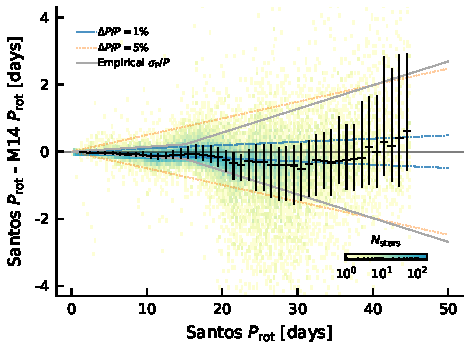
\includegraphics[width=0.48\textwidth]{perioddiff_vs_period_diffProt-m14_Prot_vs_Prot.pdf}
      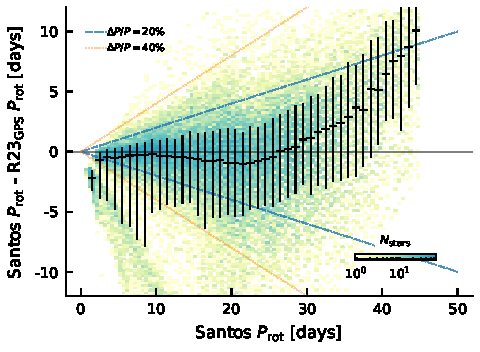
\includegraphics[width=0.48\textwidth]{perioddiff_vs_period_diffProt-r23_ProtGPS_vs_Prot.pdf}
  \end{center}
  \vspace{-0.6cm}
  \caption{
    {\bf Comparison of reported literature stellar rotation periods}.
    ``Santos'' refers to the concatenation of \citet{Santos_2019} and
    \citet{Santos_2021}.  ``M14'' refers to \citet{McQuillan_2014}.
    ``R23$_{\rm GPS}$'' refers to the Gradient of Power Spectrum
    periods from \citet{Reinhold2023}.  The background is a 2-D
    histogram with a logarithmic color stretch that counts overlapping
    stars between these studies.  The black errorbars show the median
    and $\pm$1$\sigma$ range of period the differences in 1-day bins.
    The
    solid gray ``empirical $\sigma_{\rm P}/P$'' line in the left panel
    shows the expected $\pm 1\sigma$ range that would be spanned if
    the indepndent $P_{\rm rot}$ measurements had gaussian
    uncertainties drawn following the empirical estimate described in
    Section~\ref{subsec:rotsel}.
    Note the different vertical scales.
    \label{fig:perioddiff}
  }
\end{figure*}

While we opted for the \citetalias{Santos_2019} and
\citetalias{Santos_2021} rotation period catalogs, the recent
analysis by \citet{Reinhold2023} bears comment.  \citet{Reinhold2023}
used a similar selection function as \citeauthor{Santos_2021}
(all Kepler stars), and considered a novel period measurement
approach based on the gradient of the power spectrum (GPS).  Their method
likely provides greater completeness, due to its greater sensitivity
to signals that are only weakly periodic.  

Figure~\ref{fig:perioddiff} shows histograms of the differences
between reported periods from these various studies.  The left panel
compares overlapping stars from \citet{McQuillan_2014} and
the \citeauthor{Santos_2021} studies.  The periods agree at a precision of
$\lesssim$0.01$P_{\rm rot}$ for $P_{\rm rot}\lesssim$15\,days, and at
$\lesssim$0.03$P_{\rm rot}$ for $P_{\rm rot}\approx$30\,days.  
A small bias exists at $P_{\rm rot}$$\approx$10\,days,
in the sense that the Santos periods tend to be $\approx$1\% faster
for such stars.

The right panel compares overlapping periods from the
\citet{Reinhold2023} GPS method and the \citeauthor{Santos_2021} studies.  The
periods agree at a precision of $\lesssim$0.20$P_{\rm rot}$ for
$P_{\rm rot}\lesssim$15\,days, and at $\lesssim$0.30$P_{\rm rot}$ for
$P_{\rm rot}\approx$30\,days.  A  bias develops past $P_{\rm
rot}\gtrsim$30\,days, in the sense that the \citeauthor{Santos_2021}
periods tend to be 10-20\% longer than the GPS periods.  The origin of
this larger scatter could be connected to the need for the GPS method
to determine the ``$\alpha$ calibration factor'', which is known only
at a statistical level for large stellar populations
\citep[see][]{Reinhold2023}.  While we considered deriving independent
rotation-based ages using the \citet{Reinhold2023} GPS periods with an
inflated empirical uncertainty, we ultimately opted against this path.
A rotation period difference of 20-30\% away from the ``true period''
could sufficiently skew a star's age that we prefer to restrict our
attention to the stars for which precision is a possible
outcome.





\section{Defining An ``Isochronally Far From The Main Sequence'' Boundary}
\label{app:linemethod}

The (arbitrary) method used to construct the orange line in 
the lower panel of Figure~\ref{fig:stellarprops} was as follows.
The line is	defined as
the maximum of two numerically-determined functions, $f_0(T_{\rm eff})$ and $f_1(T_{\rm eff})$.
We defined $f_0$ by fitting an
$N^{\rm th}$-order polynomial to the stars with rotation periods for which $t_{\rm
	B20,iso}/(+\sigma_{t,{\rm B20,iso}})\approx 3$
and $T_{\rm eff}\in[3700,5900]$\,K, where
$t_{\rm B20,iso}$ was the isochronal age reported by
\citet{Berger_2020a_catalog}.  We let the order of the fit vary from
$N$=1 to 10, minimized the Bayesian Information Criterion,
and found $N$=6.  
By eye, this yielded a plausible locus for $T_{\rm eff}$$\lesssim$5300\,K.
However for F and G dwarfs, the resulting locus
allowed for stars that were ``too evolved''; the density of KOIs 
was anomalously low in this region of the $\log g$ vs.\ $T$$_{\rm eff}$ plane.
We therefore visually selected KOIs that appeared
to be near the main sequence -- i.e.~most of the yellow
points in Figure~\ref{fig:stellarprops} -- and used them to fit a separate
polynomial $f_1$ through a similar BIC-minimization procedure,
which yielded $N$=3.
This polynomial, $f_1$, is shown in very faint opacity in Figure~\ref{fig:stellarprops}.
The portion of the orange locus from $\approx$5300--6200\,K
is set as $f_1 + c$, for $c$ a constant offset that we defined to be
0.1\,dex above the ``KOI main sequence''.
The exact break-point in temperature is automatically set by ${\rm max}(f_0, f_1+c)$.
While we do report rotation-based ages for stars
above this orange locus,
they are flagged as not being near the main sequence in the $\log g$ vs.~$T_{\rm eff}$ plane. 


\section{Cases With ``Inconsistent'' Rotation and Lithium-Based Ages}
\label{app:inconsistent}

In this section we discuss the systems with confirmed planets that
have nominally discrepant rotation and lithium-based ages.  We find
that only one of them, Kepler-786, is interesting.

\paragraph{Kepler-1}---TrES-2/Kepler-1 \citep{2006ApJ...651L..61O} is
a $\approx$2.5\,day near-grazing hot Jupiter oribiting a G0 V primary
which has been studied in detail by multiple investigators
\citep[e.g.][]{2007ApJ...664.1190S,2008ApJ...682.1283W,2011ApJ...733...36K,2011MNRAS.417.2166S}.
Our lithium-based age of this system (\trestwotli\,Myr), derived from
EW$_{\rm Li}^{\ast}$=81$\pm$3\,m\AA, qualitatively agrees with the
previously noted lithium abundance \citep{2007ApJ...664.1190S}.
However, we detect no photometric rotation signal, and the
spectroscopic $v\sin i$ is low.  The lithium age is strongly
asymmetric because of the scatter in EW$_{\rm Li}$ vs.~$T_{\rm eff}$
over ages $t$$\gtrsim$1\,Gyr for early G dwarfs.  We calculate a
$2\sigma$ upper limit on $t_{\rm Li}$ of 2.8\,Gyr, and a $3\sigma$
upper limit of 6.1\,Gyr.  The non-detection of rotation, while mildly
surprising, is not shocking if the system's true age is in this long
tail.

\paragraph{Kepler-101}---This $\approx$5500\,K star has EW$_{\rm
Li}^{\ast}$=100$\pm$5\,m\AA, nominally implying $t_{\rm
Li}$$\approx$200-800\,Myr, but no rotation detection.  Our automated
flags noted that this star has a low surface gravity, high luminosity,
and is far from the main sequence.  \citet{2014A&A...572A...2B}
concur: this star is a sub-giant slightly more massive than the Sun;
no rotation detection is expected; the lithium likely simply survived
over the star's main sequence lifetime.

\paragraph{Kepler-108}---This system of two mutually inclined giant
planets \citep{2017AJ....153...45M} has a $T_{\rm
eff}$$\approx$5600\,K host star with a strong lithium detection, and
no rotation detection.  The host star is entering the red giant
branch; this has been previously noted through asteroseismology
\citep{2013ApJ...767..127H}, and our analysis of the Keck/HIRES
spectrum with \texttt{SpecMatch-Synth} \citep{2017AJ....154..107P}
concurs, yielding $T_{\rm eff}$=5668$\pm$100\,K, $\log g$=3.8$\pm$0.1,
[Fe/H]=0.38$\pm$0.06, and $v\sin i$=3.2$\pm$1.0\kms.  Given the star's
high mass, the high lithium content and lack of rotation detection is
not surprising.

%Independently, Kepler~108 was also reported by \citet{2020ApJ...903...55P} to be a member
%of NGC6811.  The cluster has $\mu_\alpha\approx-3.4$mas/yr and
%$\mu_\delta \approx -8.8$mas/yr.  Kepler~108 has
%$\mu_\alpha=-1.5\pm0.1$\,mas/yr and $\mu_\delta \approx
%-1.2\pm0.1$\,mas/yr \citep{Gaia_DR3_2022}.  We therefore suggest that it is not a member
%of NGC6811.


\paragraph{Kepler-786}---This K3 V star has a surprisingly high
lithium content.  The spectrum is single-lined, with
\texttt{SpecMatch-Synth} derived parameters of $T_{\rm
eff}$=4769$\pm$100\,K, $\log g$=4.5$\pm$0.1, [Fe/H]=0.11$\pm$0.06, and
$v\sin i$=2.4$\pm$0.6\kms.  Yet with EW$_{\rm
Li}^{\ast}$=83$\pm$6\,m\AA, the lithium age of \kepseveneightsix\,Myr
would predict an obvious rotation signal.  None is present in the
Kepler light curve, consistent with the low $v\sin i$.  Out of all
``apparently discrepant'' lithium and rotation measurements discussed
in this appendix, this is the only one that seems to remain discrepant
after scrutiny.  The  \ion{Ca}{2} doublet is in emission, with
$R'_{\rm HK}=-4.7\pm0.5$, which suggests an age at least as old as the
Hyades \citep{Mamajek_2008}.  The Balmer lines are in absorption, and
display no obvious signatures of youth.


\paragraph{Kepler-1644}---The rotation-based age of this system
(\kepsixteenfourfour\,Myr) is nominally much lower than the lithium
limit ($>$767\,Myr).  The Kepler light curve shows a $\approx$1\%
amplitude 1.4\,day rotation signal with many flares.  However the
automated quality flags note that the star has low (photometric)
surface gravity, a high RUWE (${\rm RUWE}_{\rm DR3}$=7.0), and that it
is far from the main sequence.  The Keck/HIRES spectrum also shows
visually narrow lines, with a \texttt{SpecMatch-Synth} $v \sin i \leq
2$\kms.  However, we performed a cross-correlation between the HIRES
spectrum and the nearest matches in the Keck/HIRES template library
\citep{2015AJ....149...18K}, and found that on 31 July 2022 (UT) the
system displayed a broad CCF with a blended second component at
$\approx$$+26$\,\kms relative to the primary, with a best-fit
flux-ratio of $\approx$3.4\%, and a preferred $T_{\rm
eff,B}$$\approx$4400\,K.  The spectrum and astrometric excess noise
therefore point to this system being an unresolved binary, which calls
the reliability of the rotation-based age into question.  The
non-detection of the companion from Robo-AO imaging at Palomar
\citep{2017AJ....153...66Z} suggests that the companion(s) are likely
within $\rho$$\lesssim$0.3$''$.



\paragraph{Kepler-1699}---This system is in a similar qualitative
regime as Kepler-1644, with an apparently young $t_{\rm
gyro}$=\kepsixteenninenine\,Myr derived from a $\approx$2\% amplitude
4.2\,day rotation signal, and no evidence for lithium.  The system has
${\rm RUWE}_{\rm DR3}$=19.1.  From the same style of CCF analysis from
the Keck/HIRES spectrum acquired on 31 Aug 2022 (UT), we also find a
double-peaked CCF, in this case with a secondary component at
$\approx$$-16$\,\kms relative to the primary with $T_{\rm
eff,B}$$\approx$4900\,K.  This putative companion is similarly not
detected in high-resolution imaging \citep{2017AJ....153...66Z}.  The
rotation-based age is questionable, given that we do not know which
source the rotation signal is from, or whether the stars have
interacted.

\paragraph{Kepler-1943}---This system nominally has a
\kepnineteenfourthree\,Myr lithium age, and no reported rotation
detection.  However, the star is flagged as being over-luminous,
low-surface gravity, and far from the main sequence.  In other words,
it is a subgiant.

\paragraph{Kepler-639, Kepler-320, Kepler-1719, Kepler-1876,
Kepler-1072, Kepler-1743, Kepler-1929, Kepler-1488}---These eight
systems all have nominally two-sided lithium age posteriors between 1
and 3\,Gyr, and yet lack rotation period detections.  All are
subgiants, flagged with $Q_{\rm star}$ under various combinations of
bits 1, 2, and 9.


\section{Notes on Individual Systems}

%Kepler~221 is a 633$^{+120}_{-112}$\,Myr four-planet system.
%
%Kepler~51 (CITE Masuda2014) has previously been noted for its bizarre architure.
%The rotation-based age we find here is higher/lower than previously noted.

Kepler~411, a $t_{\rm gyro}$$\approx$780$\pm$170\,Myr early K dwarf with three
transiting planets at 3.0, 7.8, and 58\,days, has a rare
architecture.  \citet{2019A&A...624A..15S} conducted a transiting
timing analysis of the system, confirming Kepler-411d and arguing for
the presence of a fourth non-transiting planet, Kepler-411e, based on
the TTVs seen in Kepler-411d and assuming that the system is nearly
coplanar.  Regarding the stellar age, \citet{2019A&A...624A..15S} used
the \citet{2007ApJ...669.1167B} relation and the measured rotation
period, which yielded an estimate of 212$\pm$31\,Myr.  However, the
star's temperature ($\approx$4900\,K) puts it in a regime where the
\citeauthor{2007ApJ...669.1167B} relation has been known to not fit
observations for a while
\citep[e.g.][Fig.~9]{Mamajek_2008}.  Our adopted age of
$\approx$780$\pm$170\,Myr agrees with the open cluster calibrators.

%\section{TODO's}
%
%\begin{enumerate}
%%  \item Compare Mathur2023 ages against my ages, and (more interestingly) against the
%%    cluster scale using NGC6811, Theia520, Melange3, and CepHer stars.
%%    Could compare against asteroseis too.
%%    %
%%  \item Intro needs better discussion of Mathur2023 and Lu2021
%    %
%  \item Consider moving the bit list description to its own appendix.
%    %
%  \item Rerun gyro calculation with denser grid, fixing quantization
%    and extending upper limit to 5gyr.  (Will use updated Teff
%    uncertainties)
%\end{enumerate}


%\section{Comparison Against Previous Literature Age Scales}
%Searching the literature for gyrochronal analyses of the Kepler field,
%the most relevant studies seemed to be those of
%\citet{Walkowicz_2013}, \citet{Reinhold_2015}, and 
%\citet{David_2021}.
%
%Also Mathur2023, which does ``magneto-gyrochronology'', including the
%Sph indicator in a model of the ages.
%
%
%\subsection{Asteroseismic Age Comparison}
%T Ceillier, J Van Saders et al 2016 MNRAS...



\section{Age Diagnostics}
\label{app:age_diagnostic}

Figure~\ref{fig:gyroage_vs_teff} is a visualization of $t_{\rm gyro}$
vs.~$T_{\rm eff}$ for our rotation-based age catalog. 
Each bar denotes the $\pm$1$\sigma$ uncertainty for a star's
rotation-based age:
this plot can be viewed as the transformation of
the left panel of Figure~\ref{fig:prot_vs_teff}.
The overdensity of $P_{\rm rot}$$\approx$20\,day G dwarfs corresponds
to the large overdensity at $t_{\rm gyro}$$\approx$3\,Gyr.
The (non-physical) deficit of $\sim$22\,day rotators appears as a
deficit between 5500--6000\,K.
A second deficit is also visible from 3800--5000\,K;
it is associated with the ``intermediate period gap'', which may be
associated with a transition from spot-dominated to faculae-dominated
light curves \citep[e.g.][]{Reinhold2019}.
At $\approx$1\,Gyr, stalled spin-down yields larger uncertainties for
K dwarfs.
The pile-up near $\approx$5\,Gyr is imposed by our choice of prior;
given that \texttt{gyro-interp} returns non-calibrated ages in this
regime, we truncated our analysis at 4\,Gyr.

\begin{figure*}[!t]
  \begin{center}
    \leavevmode
        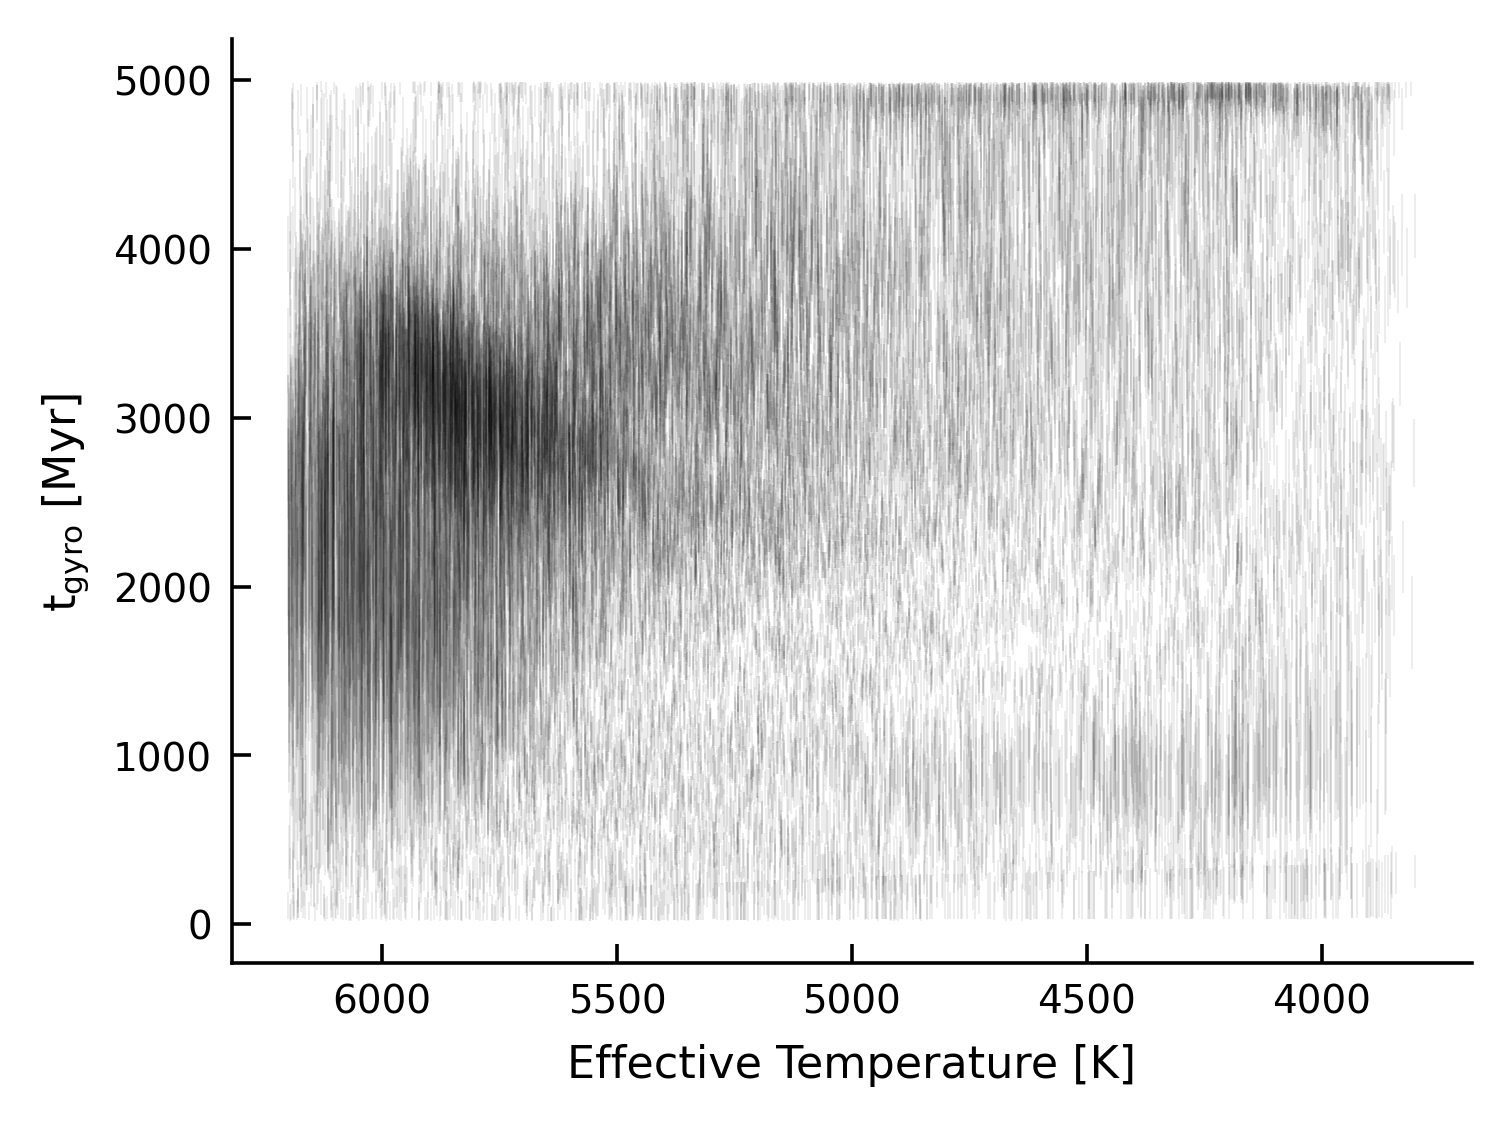
\includegraphics[width=0.48\textwidth]{gyroage_vs_teff_errs_linear.png}
    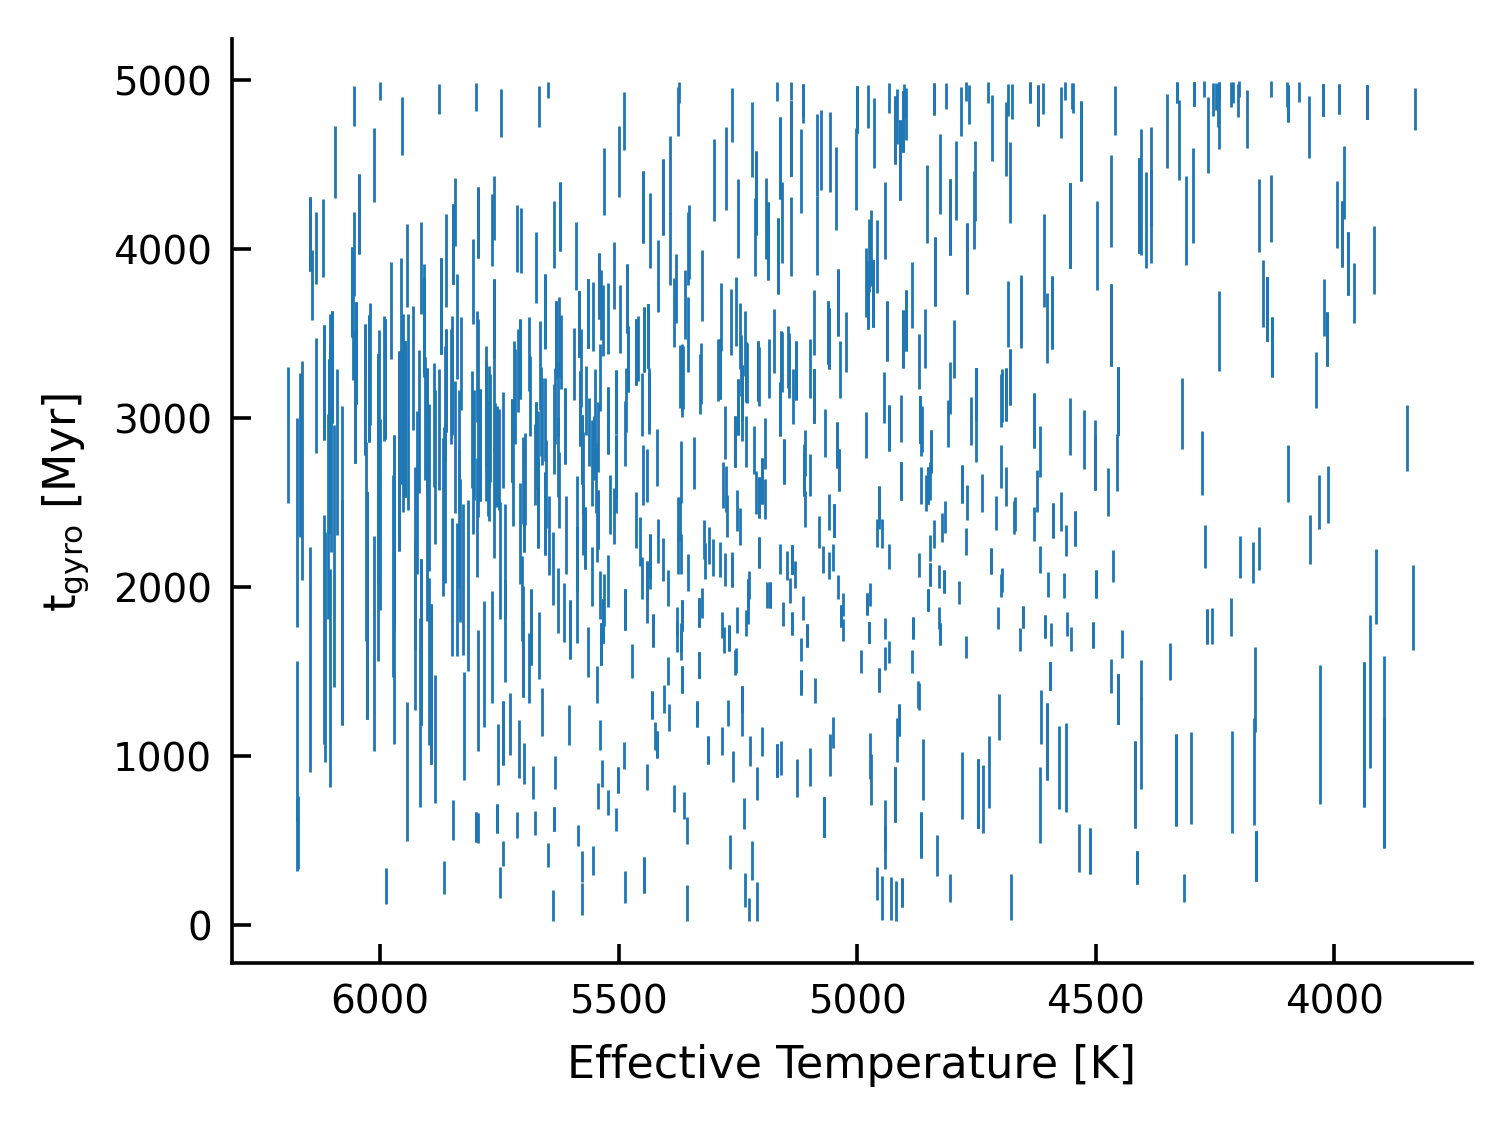
\includegraphics[width=0.48\textwidth]{gyroage_vs_teff_errs_showplanets_linear.png}
  \end{center}
  \vspace{-0.6cm}
  \caption{
    {\bf Rotation-based age vs.~effective temperature}.
    The entire Kepler sample is shown on the left.
    KOI hosts are shown on the right.
    Each bar shows the $\pm$1$\sigma$ uncertainty for a star's age as
    derived from its rotation period.  
    Notable features are discussed in
    Appendix~\ref{app:age_diagnostic}.
    \label{fig:gyroage_vs_teff}
  }
\end{figure*}

\clearpage
\listofchanges

\end{document}
